% Based on the official CVPR 2027 author kit, tag CVPR2027-v1.
\documentclass[10pt,twocolumn,letterpaper]{article}

\usepackage[review]{cvpr}
% Use \usepackage{cvpr} instead for the camera-ready version.
% !TeX root = main.tex
%% This file contains a number of tweaks that are typically applied to the main document.
%% They are not enabled by default, but can be enabled by uncommenting the relevant lines.


%%
%% Official support for 2-column teaser figure
%%
\usepackage{cuted} %< for strip environment

%%
%% For auto-referencing of figures (see fig/teaser.tex and \label{} therein) 
%%
\usepackage{currfile} %< for \currfilebase macro
\usepackage{microtype}
\usepackage{array}
\usepackage{xspace}
\newcommand{\method}{HereWeChoreography\xspace}

%%
%% caption and (global) spacing overrides
%%
\usepackage{caption} %< for "\captionof" commands (teaser)
% \setlength{\abovecaptionskip}{.5em} % space above caption
% \setlength{\belowcaptionskip}{1em} % space below caption

%%
%% Inline annotations; for predefined colors, refer to "dvipsnames" in the xcolor package:
%% https://tinyurl.com/overleaf-colors
%%
\newcommand{\red}[1]{{\color{red}#1}}
\newcommand{\todo}[1]{{\color{red}#1}}
\newcommand{\TODO}[1]{\textbf{\color{red}[TODO: #1]}}
%%
%% Disable for camera ready / submission by uncommenting these lines:
%%
% \renewcommand{\TODO}[1]{}
% \renewcommand{\todo}[1]{#1}

%%
%% Work harder in optimizing text layout. Typically shrinks text by 1/6 of page, enable
%% it at the very end of the writing process, when you are just above the page limit.
%%
% \usepackage{microtype}

%%
%% Fine-tune paragraph spacing.
%%
% \renewcommand{\paragraph}[1]{\vspace{.5em}\noindent\textbf{#1.}}

%%
%% Globally adjusts space between figure and caption.
%%
% \setlength{\abovecaptionskip}{.5em}

%%
%% Allows "the use of \paper to refer to the project name"
%% with automatic management of space at the end of the word.
%%
% \usepackage{xspace}
% \newcommand{\paper}{ProjectName\xspace}

%%
%% Commonly used math definitions.
%%
% \DeclareMathOperator*{\argmin}{arg\,min}
% \DeclareMathOperator*{\argmax}{arg\,max}

%%
%% Tighten underline.
%%
% \usepackage{soul}
% \setuldepth{foobar}

%%
%% Reconfigure paragraph (tweaks spacing)
%%


\definecolor{cvprblue}{rgb}{0.21,0.49,0.74}
\usepackage[pagebackref,breaklinks,colorlinks,allcolors=cvprblue]{hyperref}

\def\confName{CVPR}
\def\confYear{2027}
\def\paperID{1134}

\title{HereWeChoreography: From Motion Primitives to Long-Form Choreography}
\author{Anonymous CVPR submission}

\begin{document}
\maketitle

% !TeX root = ../main.tex
\begin{abstract}
Music-to-text choreography represents a dance as an inspectable, timed
movement score. It requires actionable local descriptions, coherent
whole-song organization, and evaluation that admits multiple valid dances
for the same music. We introduce \method through an evidence-linked
annotation resource, a dedicated model trained by supervised fine-tuning,
a compositional harness, and a multi-level evaluation protocol. The
design decouples local movement prediction from global composition:
short-clip proposals are organized into bar-aligned units using musical
evidence, global style, segment objectives, and motif memory. Schedule
validation and bounded revision preserve accepted context. Source-event
links make annotation refinement auditable. On a frozen 2,000-clip panel, the adapted
model achieves 30.80 ROUGE-L versus 14.99 for the best evaluated general
audio-language baseline on this metric, demonstrating stronger reference
agreement. Our evaluation protocol separately addresses local musical
response and whole-song organization. Preliminary whole-song results
concern the historical fixed-window harness; controlled comparison of
the latest bar-aligned agents and independent audio-grounded assessment
remain prospective.
\end{abstract}

% !TeX root = ../main.tex
\section{Introduction}
\label{sec:introduction}
Music-to-text choreography takes a musical recording and produces a
timed score of movements. Such a score makes compositional decisions
inspectable and editable before performance or rendering. Music-conditioned
dance generators synthesize motion sequences~\cite{aistpp,bailando,edge};
we study the textual planning interface, where movement content, its
ordering, and its development across a song must be stated explicitly.

This task presents three requirements. First, descriptions must specify
actionable movements rather than merely characterize the music. Training
them requires movement supervision with traceable source evidence.
Second, locally plausible actions must form a composition: independent
short-clip predictions do not determine transitions, motif recurrence,
or progression over an entire song. Third, evaluation must accommodate
multiple valid dances for the same music. Agreement with one recorded
dance therefore measures only part of the task; musical response and
whole-song organization require separate assessment.

We address these requirements with \method, which decouples local movement
prediction from global composition. A dedicated short-clip model provides
movement proposals. A stateful harness groups two to four musical bars
into duration-aware units and composes them using a segment outline,
shared musical evidence, a global dance-style condition, and accepted
history. Motif memory tracks recurrence and variation. Schedule validation
precedes commitment, while bounded revision targets repetitive action
spans and preserves their temporal scaffold. The outer planner operates
with fixed model weights.

The framework delivers an evidence-linked annotation resource and
construction pipeline, a task-specific model trained by supervised
fine-tuning, a compositional harness, and an evaluation protocol with
six local and three whole-song dimensions. Current experimental captions
refine 2D rule logs using GPT-6.1-sol; the implemented geometry-aware 3D
annotation route remains an extension. The evaluation protocol requests
explicit textual and musical evidence, separating reference agreement
from judgments of choreography quality.

On a frozen 2,000-clip panel, the adapted model achieves 30.80 ROUGE-L,
compared with 14.99 for the best evaluated general audio-language baseline
on this metric. These results characterize reference agreement;
music-conditioned quality requires separate assessment. Whole-song results use the historical
fixed-window harness; controlled comparisons of the latest bar-aligned
agents and independent audio-grounded assessment remain prospective.

% !TeX root = ../main.tex
\begin{figure*}[t]
\centering
\ifdefined\OverviewDataBenchmark
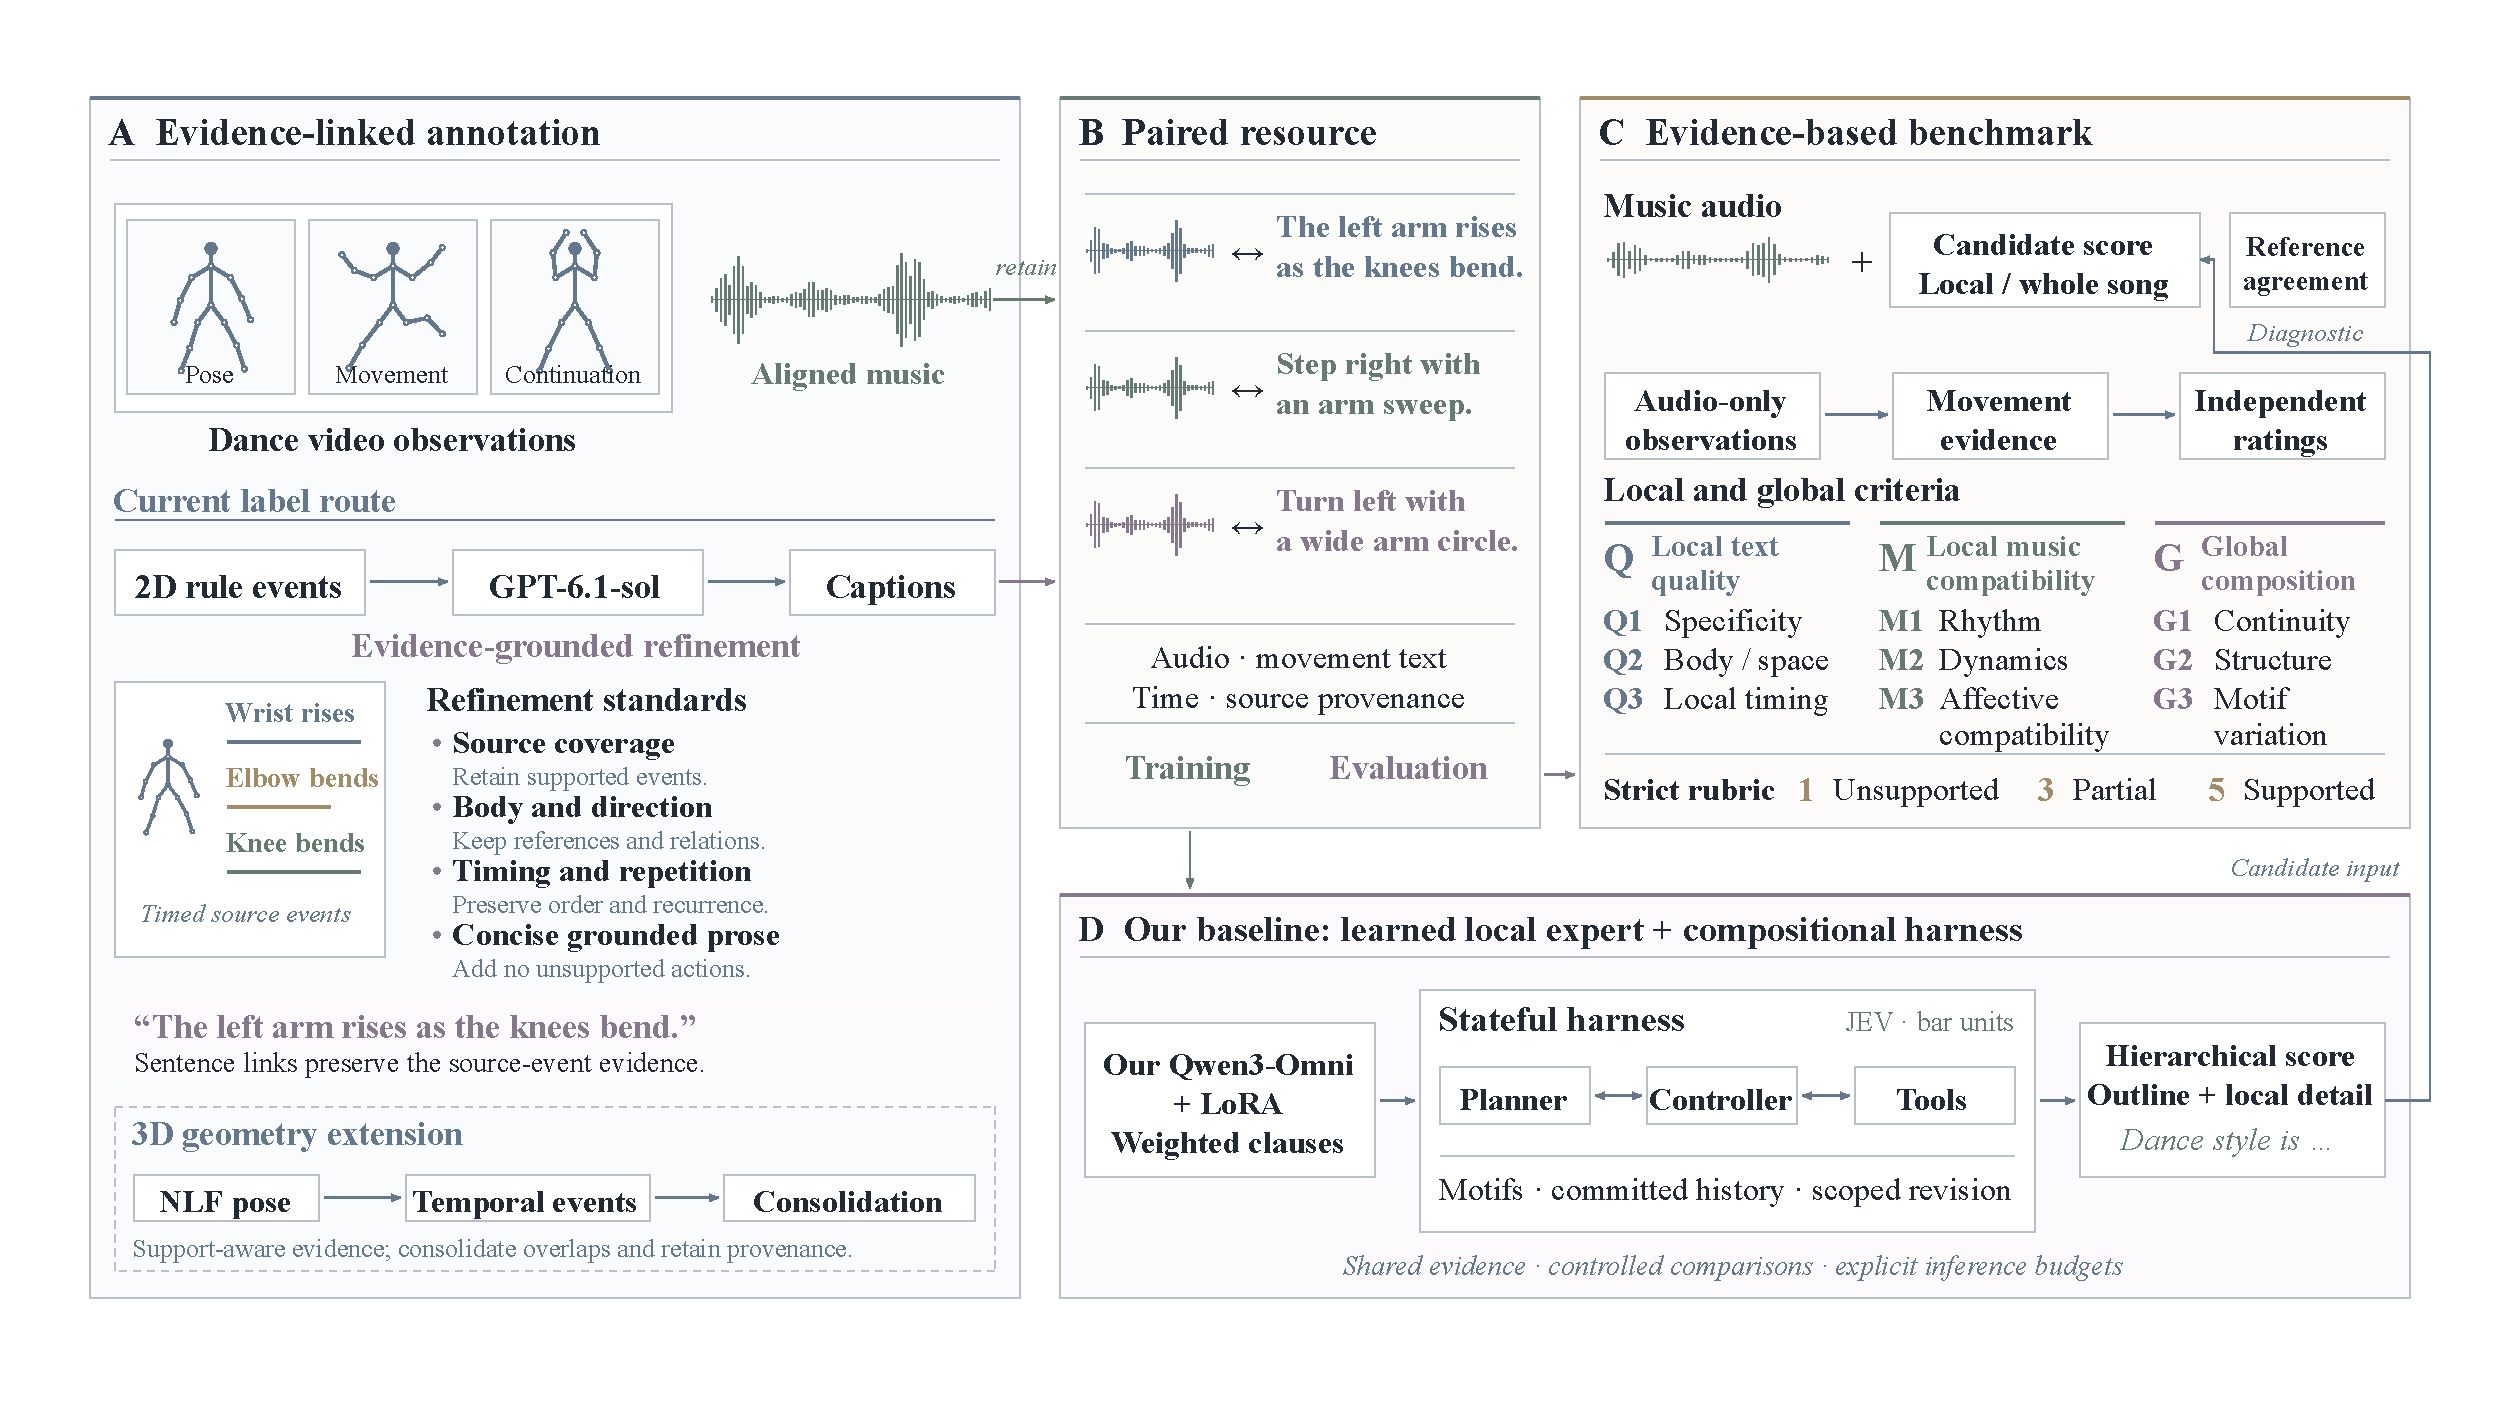
\includegraphics[width=\textwidth]{figures/revision_20261117/paper/overview_benchmark.pdf}
\caption{\textbf{Data, benchmark, and baseline in \method.}
Evidence-linked captions retain movement provenance and paired music.
Current labels follow the 2D rule-event route; the dashed 3D route
depicts the geometry extension. The trained local expert and stateful
harness provide a baseline for assessing local movement, musical
response, and whole-song composition. The proposed protocol uses audio
and quoted movement evidence; calibration remains pending.
Media, score snippets, and rubric anchors are schematic illustrations.}
\else
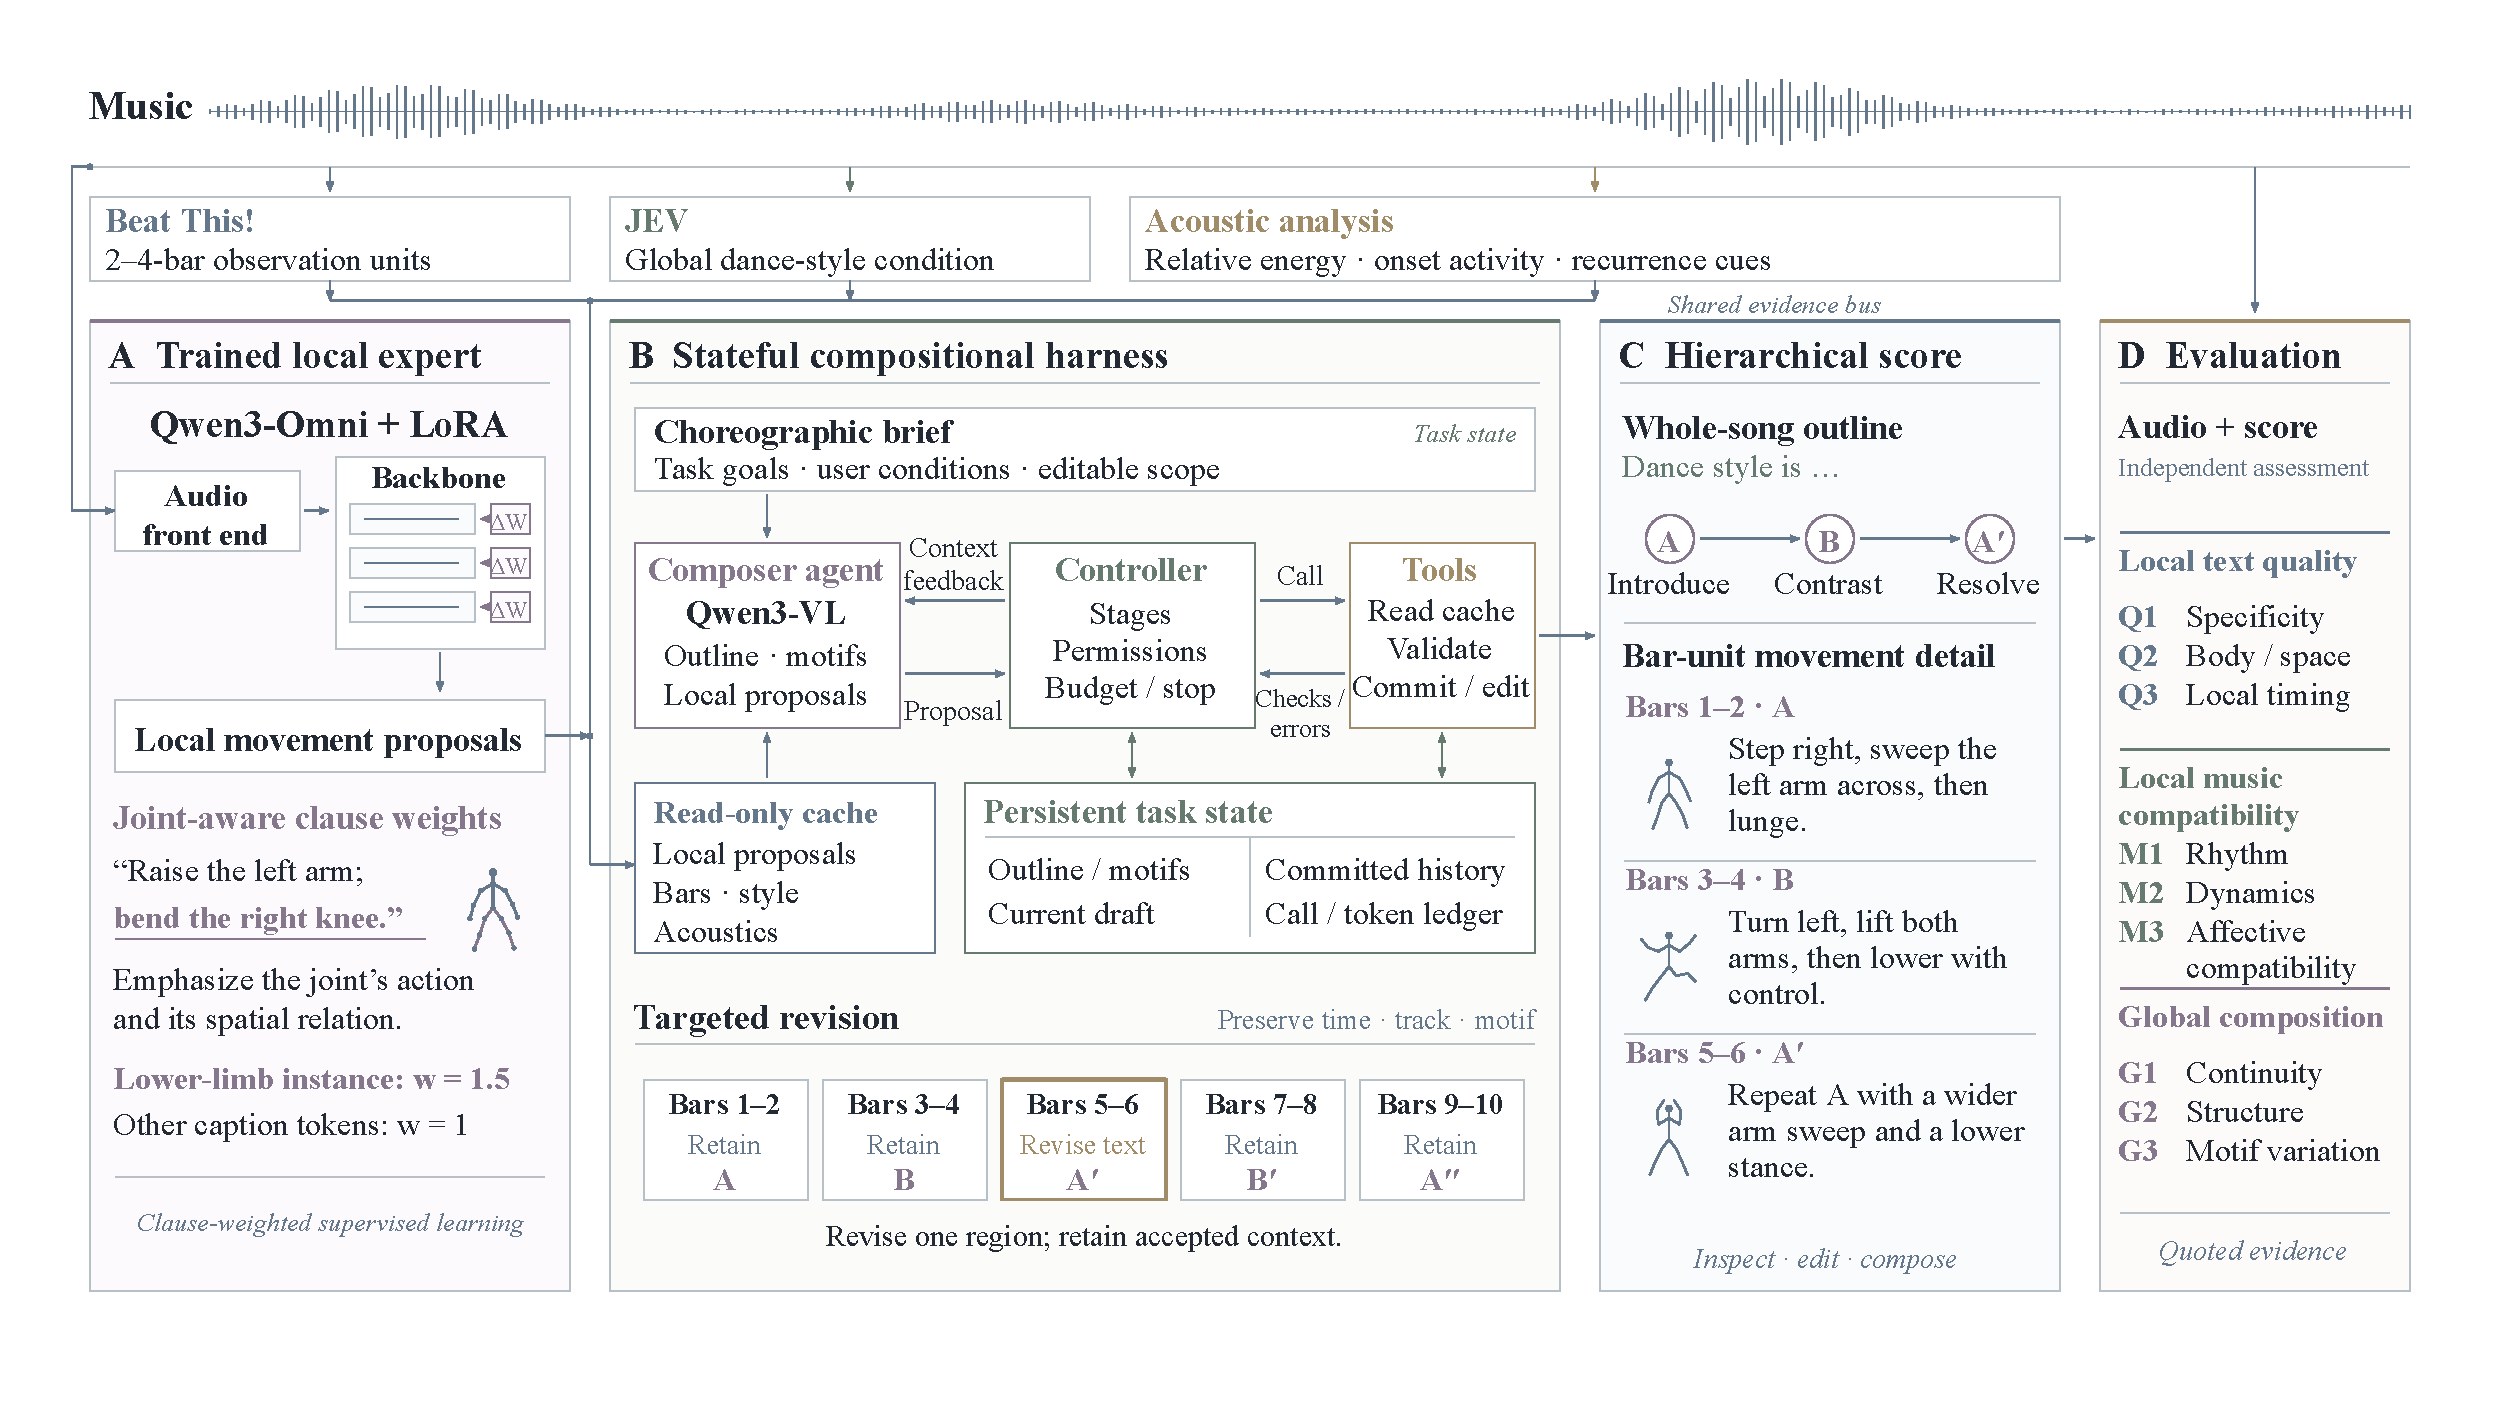
\includegraphics[width=\textwidth]{figures/revision_20261117/paper/overview_method.pdf}
\caption{\textbf{From a trained local expert to stateful composition.}
Joint-aware clause supervision trains our Qwen3-Omni expert; Beat This!,
JEV, and acoustic analysis provide shared musical conditions.
The composer proposes movements, the controller schedules tool
execution, and structural feedback informs subsequent decisions.
The task brief and persistent state retain objectives, drafts, motifs,
committed history, and budgets.
Targeted revision protects the temporal scaffold and accepted context.
The hierarchical score supports separate local and global assessment
outside the generation loop. Poses and score excerpts are schematic. The latest design uses bar
groups; reported whole-song results retain their fixed-window configuration.}
\fi
\label{fig:harness-overview}
\end{figure*}


% !TeX root = ../main.tex
\section{Related Work}
\label{sec:related-work}
\paragraph{Music-conditioned dance and language guidance.}
FACT generates long motion sequences using a cross-modal
transformer~\cite{aistpp}; Bailando composes quantized movements with
choreographic memory~\cite{bailando}; EDGE supports editable dance through
diffusion and temporal constraints~\cite{edge}. Their joint trajectories
permit evaluation of realized movement and alignment. Text already
connects music and motion: M$^3$GPT includes music-to-text
tasks~\cite{m3gpt}, and DanceChat supplies LLM-generated movement
instructions to diffusion~\cite{dancechat}. We study the textual score
itself, emphasizing whole-song composition and assessment.

\paragraph{Movement description and musical evidence.}
HumanML3D pairs motion with natural-language
descriptions~\cite{humanml3d}. MotionScript derives descriptions from
geometric attributes and temporal changes~\cite{motionscript}; NLF
localizes arbitrary body points and supports parametric
fitting~\cite{nlf}. Beat This estimates beats and
downbeats~\cite{beatthis}, MuQ provides music
representations~\cite{muq}, and Qwen2.5-Omni and Qwen3-Omni support
audio-to-text interaction~\cite{qwen25omni,qwen3omni}. These building
blocks support annotation, partitioning, style conditioning, and local
prediction. Whole-song composition additionally requires ordering,
recurrence, and retained context.

\paragraph{Inference-time control and assessment.}
ReAct interleaves reasoning and tool actions~\cite{react}; Self-Refine
iterates feedback and revision without retraining~\cite{selfrefine}.
For choreography, musical objectives, recurring motifs, and accepted
history must inform successive proposals. Our implemented common
interface enables controlled comparisons with shared evidence and
resource limits; the full comparison remains pending. BLEU, ROUGE, and
BERTScore measure reference agreement~\cite{bleu,rouge,bertscore}.
Complementary local and whole-song criteria assess movement content and
musical response with explicit evidence requirements.

% !TeX root = ../main.tex
\section{Evidence-Linked Choreography Supervision}
\label{sec:data}
% !TeX root = ../main.tex
\begin{figure*}[t]
\centering
\begin{subfigure}{\textwidth}
\centering
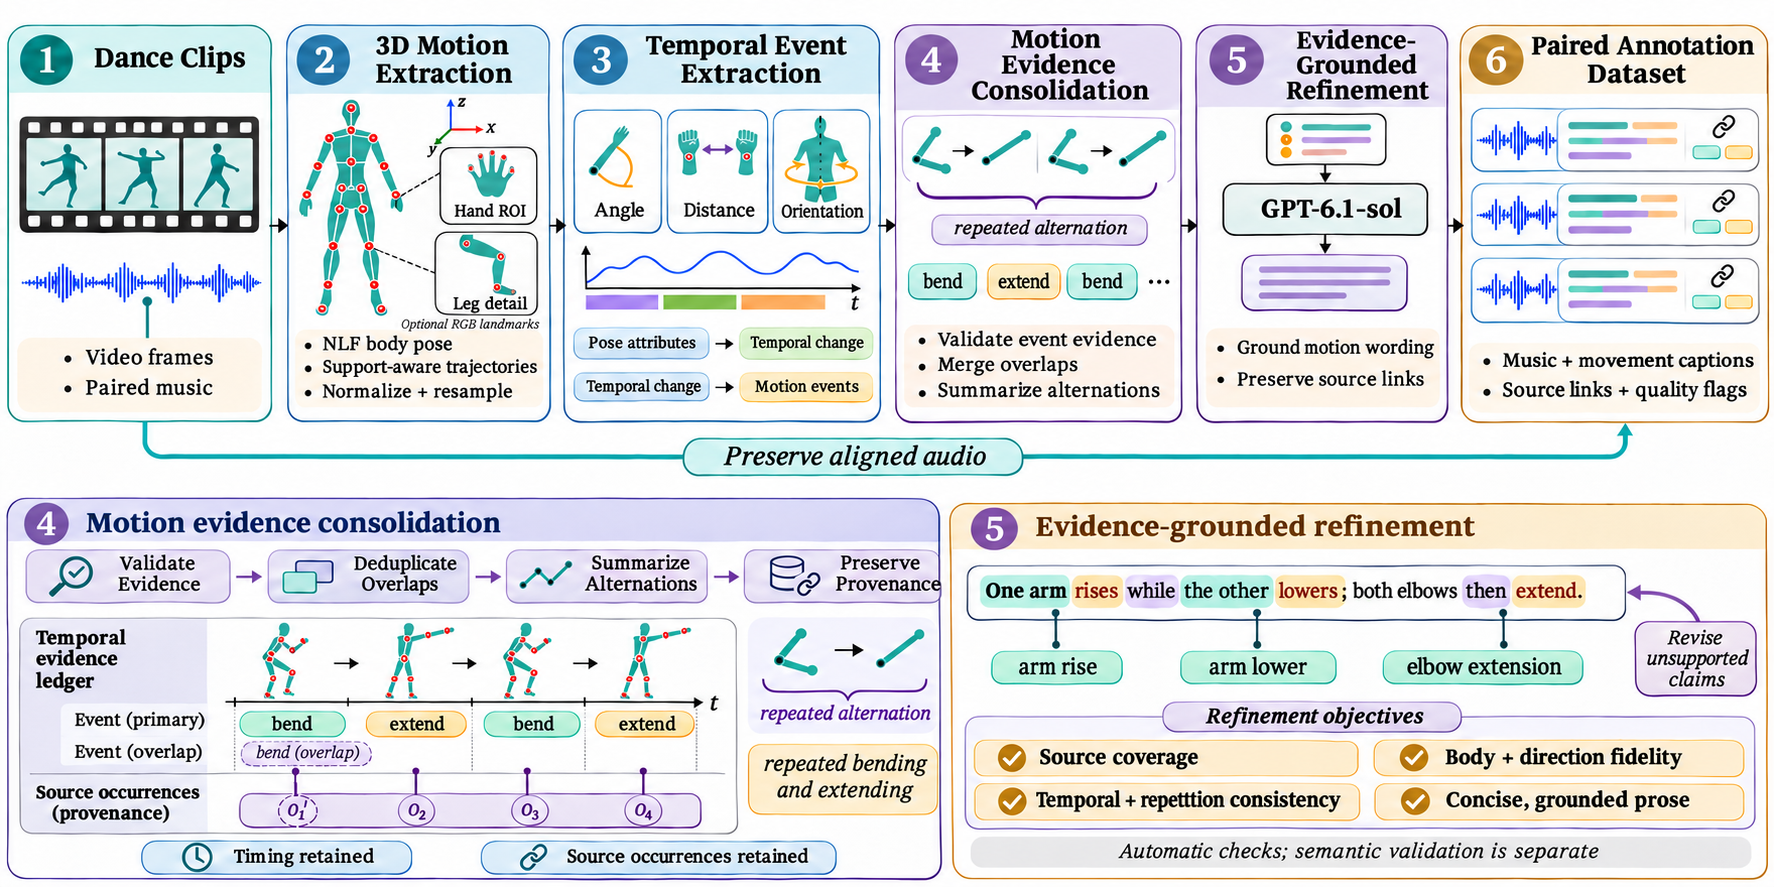
\includegraphics[width=\textwidth]{figures/annotation_pipeline_v5.png}
\caption{Geometry-based annotation framework and evidence-preserving refinement.}
\label{fig:annotation-pipeline}
\end{subfigure}
\par\medskip
\begin{subfigure}{\textwidth}
\centering
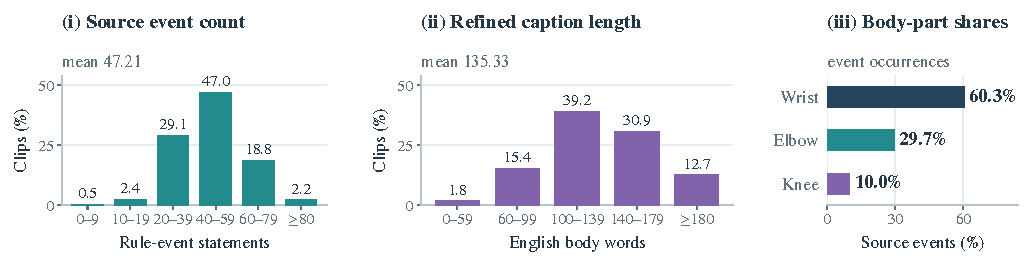
\includegraphics[width=\textwidth]{figures/annotation_distributions_v3.pdf}
\caption{Descriptive statistics on the same 22,352 paired clips.}
\label{fig:annotation-distributions}
\end{subfigure}
\caption{\textbf{Annotation construction and supervision profile.}
(a) MotionScript-based temporal extraction~\cite{motionscript},
Motion Evidence Consolidation, and GPT-6.1-sol evidence-grounded
refinement retain source occurrences and paired music. Hand/leg insets
are detail views; matching 4/5 badges identify expanded stages.
This is a component-integration framework; current experimental labels
come from the existing 2D rule-log rewrite route, detailed in
Appendix~\ref{sec:annotation-details}.
(b) Frozen paired statistics retain all automatic quality flags.
Event occurrences, caption body words, and body-part shares use different
units; they characterize supervision rather than gains in action accuracy
or diversity. The style prefix is excluded from word counts.}
\label{fig:dataset-overview}
\end{figure*}


\paragraph{Paired resource.}
The collection contains 220,667 music--choreography records, partitioned
into 198,315 training, 11,098 validation, and 11,254 test records.
Records retain media identity, observation intervals, source groups,
and annotation metadata. These inventory counts do not establish the
model's exact training subset without its training manifest; video-source
grouping likewise does not establish song-level disjointness.

\paragraph{From movement evidence to language.}
Current references are GPT-6.1-sol text-only rewrites of windowed 2D
rule-event logs: sixteen event types describe wrist directions and
projected elbow/knee angle changes. \emph{Evidence-Grounded Refinement}
targets source coverage, body/direction fidelity, timing/repetition
consistency, and concise grounded prose. Sentences link to source-event
IDs; automatic flags support auditing without human semantic approval.
The refiner receives no audio; aligned music is retained for subsequent
learning. Open-vocabulary prose remains bounded by observed events.
Figure~\ref{fig:choreography-example} illustrates how a score states body
references, movement range, and order, then carries an explicit end state
into the next action. Its author-composed instructions accompany real media.
% !TeX root = ../main.tex
\begin{figure*}[t]
\centering
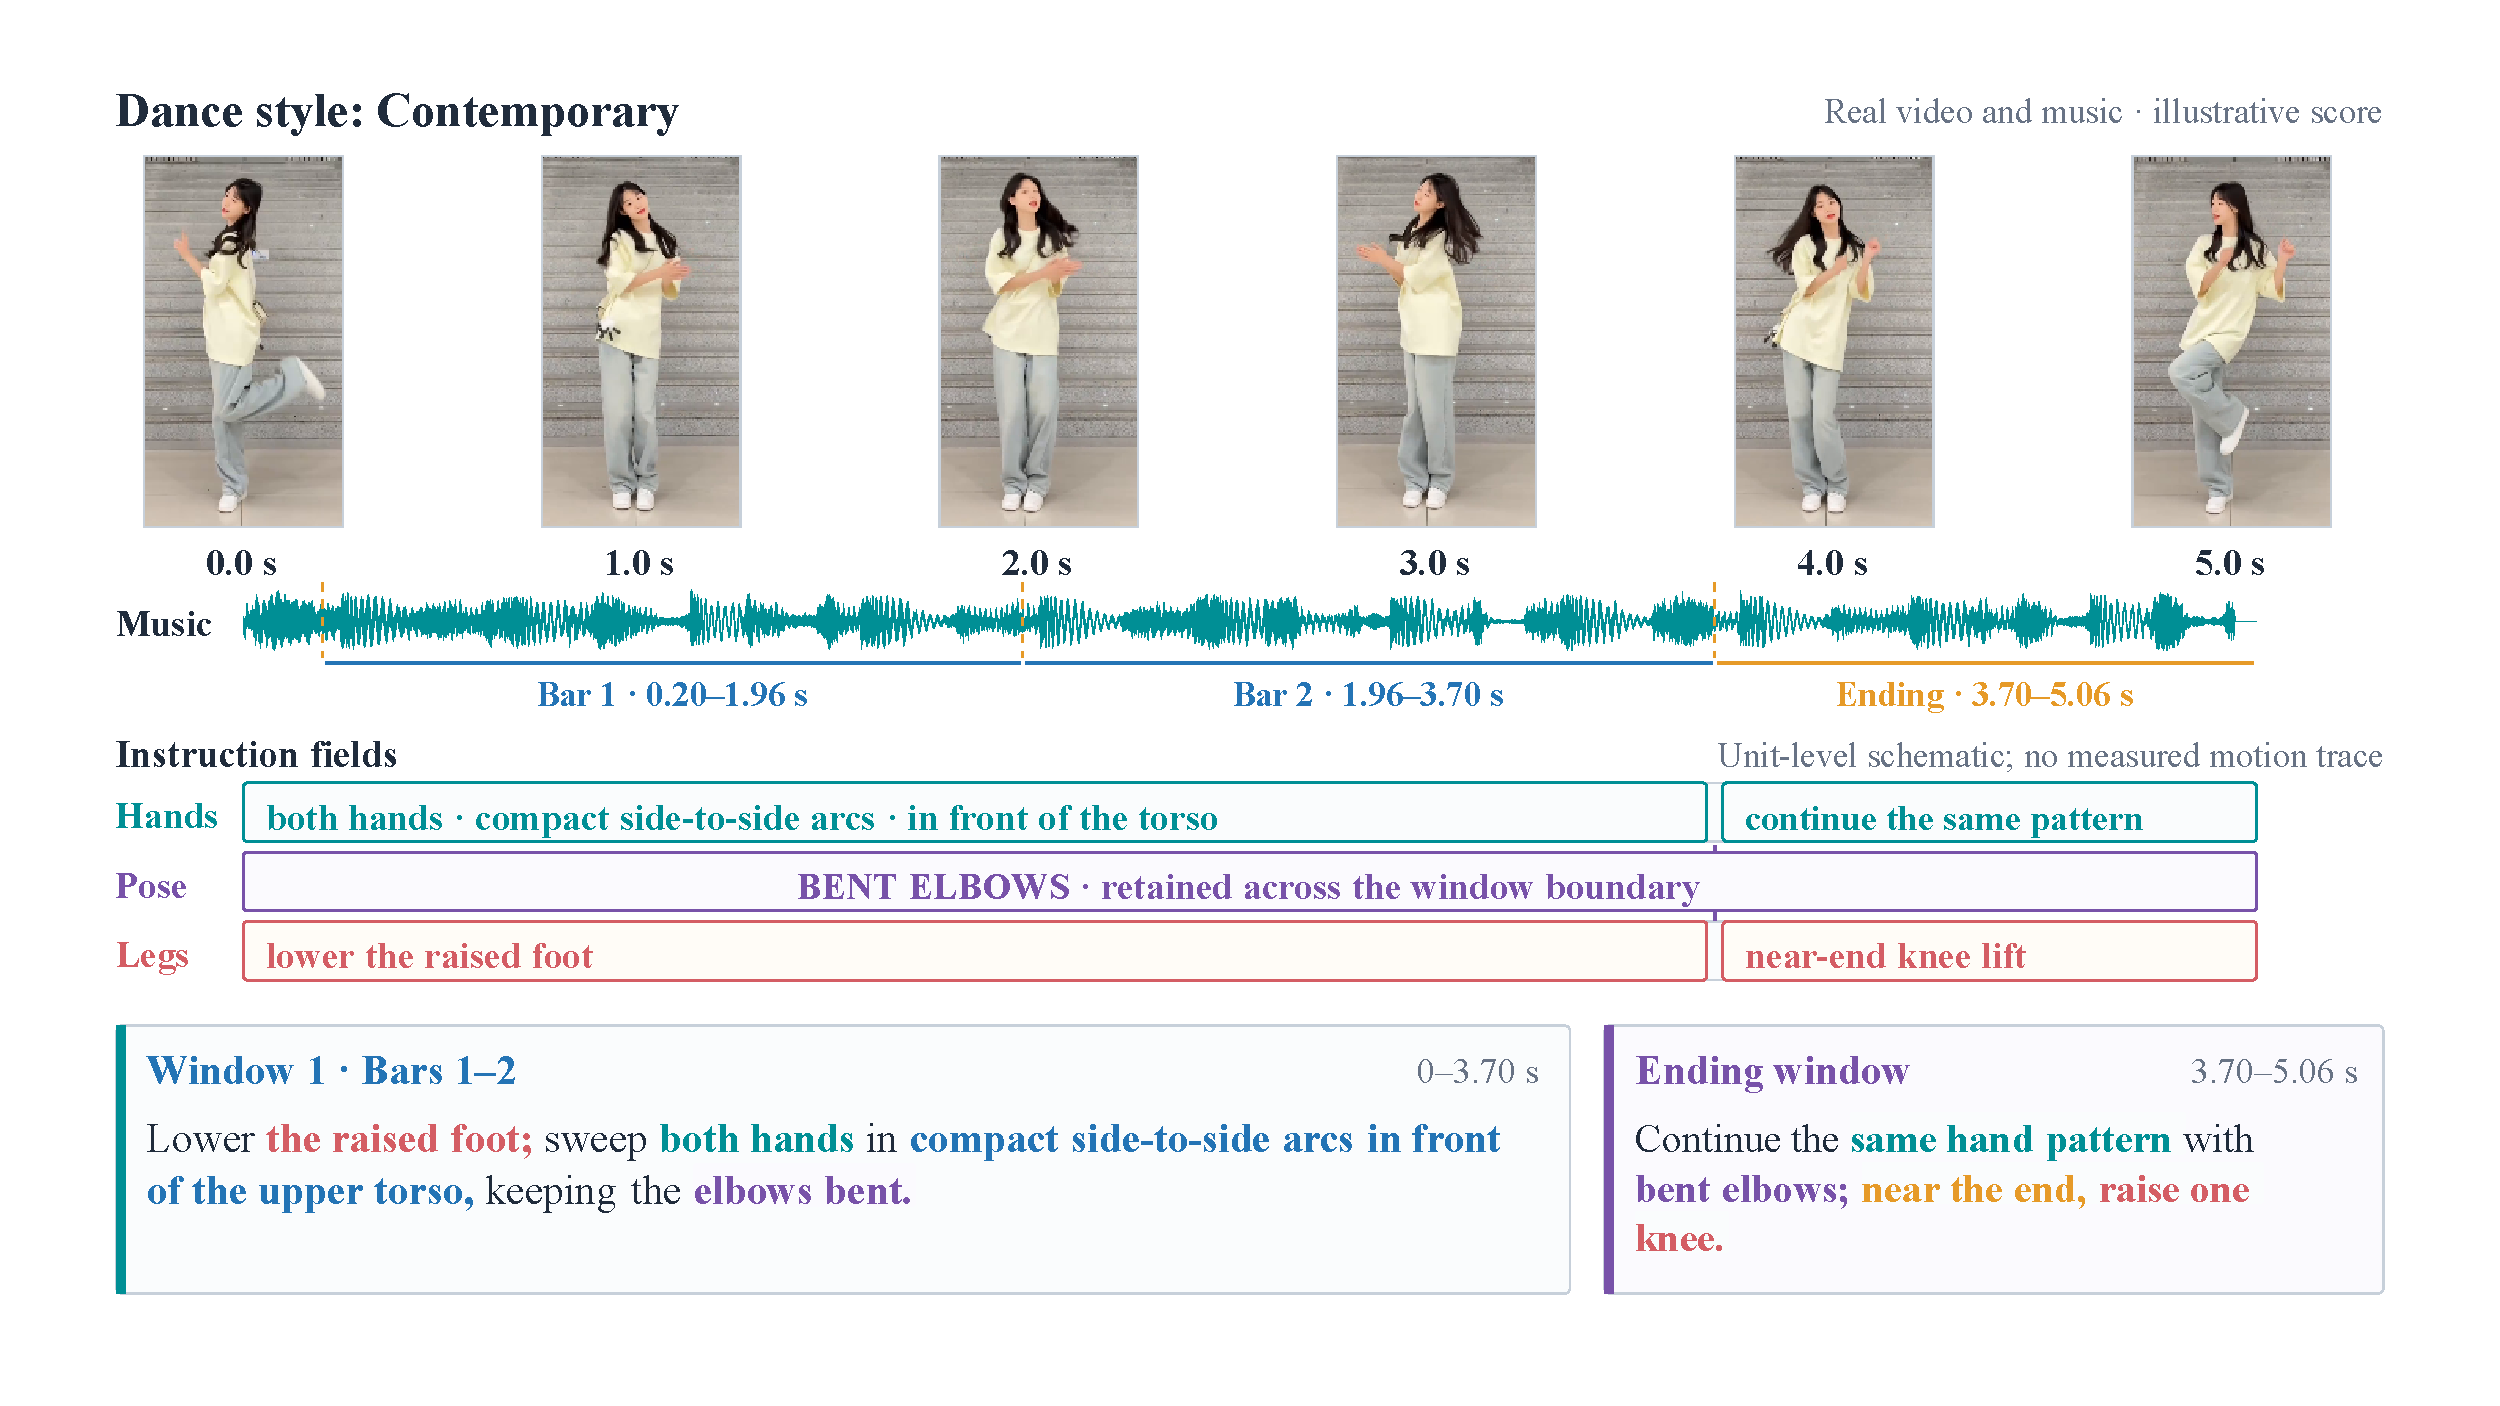
\includegraphics[width=\textwidth]{figures/revision_20261117_v3/paper/choreography_case.pdf}
\caption{\textbf{What makes a movement description informative.}
Six equally spaced real frames share a clock with the measured music
waveform. Unit-level fields expose body references, movement range and
direction, and the retained elbow state; matching colors connect these
fields to the instructions below. Predicted bars form a two-bar unit and
an ending fragment, with the initial 0--0.20\,s fragment merged.
The authored instructions and field bands illustrate the representation,
not scored predictions, measured action durations, or verified synchronization.}
\label{fig:choreography-example}
\end{figure*}


\paragraph{Geometry and evidence consolidation.}
Figure~\ref{fig:annotation-pipeline} depicts the geometry extension using
NLF~\cite{nlf} and MotionScript~\cite{motionscript}. Body-relative signals
are resampled to 20~FPS; support masks preserve unsupported intervals.
\emph{Motion Evidence Consolidation} validates evidence, deduplicates
overlaps, summarizes supported alternations, and preserves source
occurrences. Optional direct-RGB palm/foot landmarks and DWPose hand
observations supplement body geometry; template joints add no observation.
Hand insets magnify keypoints, rather than denote an implemented
independent ROI estimator. This 3D route is not established as the
production source of current labels. Appendix~\ref{sec:annotation-details}
details provenance.

\paragraph{Descriptive statistics.}
Figure~\ref{fig:annotation-distributions} compares the same 22,352 paired
validation/test clips, retaining all quality flags. Source-style metadata
are unchanged and unknown for 59.6\%. Event and word counts have
different units and do not establish greater action diversity.
References describe individual observed dances; agreement does not
imply a unique choreography for the music.

% !TeX root = ../main.tex
\section{Method}
\label{sec:method}

\subsection{Local Expert and Stateful Harness}
Given music $x$ of duration $T$ and an optional brief, we generate a whole-song textual score. Each event specifies an interval, movement track, action, and optional motif. Tracks represent concurrency; motifs represent recurring movement ideas. Our motion primitives are open-vocabulary movement proposals, rather than a learned codebook or 3D clips. Integer sample indices define the source clock; presentation and evaluation use global seconds.

The expert is a LoRA-adapted Qwen3-Omni-30B-A3B-Captioner~\cite{qwen3omni}.
We use \emph{joint-aware clause reweighting} to emphasize movement
descriptions associated with selected joints or body regions:
\begin{equation}
 \mathcal{L}_{\mathrm{SFT}}
 =-\frac{1}{N}\sum_i\sum_{t\in\mathcal V_i}
 w_{i,t}\log p_\theta(y_{i,t}\mid x_i,y_{i,<t}).
\end{equation}
Here $x_i,y_i$ are paired audio and captions, $\mathcal V_i$ contains
valid assistant tokens, and $N=\sum_i|\mathcal V_i|$.
Weights apply to text clauses, preserving supervision for the joint's
action and spatial relation. Development diagnostics identified
lower-limb omissions as a prominent failure mode; the released
configuration therefore assigns weight 1.5 to tokens in clauses naming
lower-limb parts and 1 otherwise. Its isolated causal benefit remains
to be established.

We decouple local movement prediction from long-term organization. The expert supplies $K=2$ independently requested, cached captions per window by default. A stateful harness organizes them using musical context and committed history, with all model weights fixed during inference. The controlled protocol fixes candidates, acoustic evidence, style, windows, and resource caps across strategies.

\subsection{Bar-Aligned Window Partition}
To preserve bar boundaries while keeping inputs near the expert's short training horizon, Beat This!~\cite{beatthis} supplies downbeats defining complete bars. Within each available public section, dynamic programming groups two, three, or four bars, first minimizing unavoidable singletons and then
\begin{equation}
 \sum_{u=1}^{U}(\Delta_u-\tau)^2,
 \qquad \tau=5.0625\,\mathrm{s},
\end{equation}
subject to contiguous coverage and supported durations. Actual window length is $\Delta_u$; fewer windows break remaining ties. Singletons and incomplete boundary bars are marked, with short fragments eligible for adjacent merging.

The target is soft: two $4/4$ bars at 120 BPM last four seconds. Audio duration is preserved and the timeline covered exactly once. Bars need not coincide with semantic phrases; absent functional annotations, the song forms one public section.

\subsection{Shared Musical Conditions}
Shared conditions connect local decisions to song-level context.
The JEV style expert uses a MuQ-based classifier~\cite{muq}, with
temporal mean and standard-deviation features from a frozen encoder.
Calibrated observation probabilities define global style through
\begin{equation}
 \bar{\mathbf p}=\frac{\sum_j w_j\mathbf p_j}{\sum_j w_j},
\end{equation}
where $w_j$ is attributed duration, dividing overlap equally. A supported winner yields \texttt{Dance style is <style>.} User style takes precedence; failed or unsupported predictions yield unspecified style. This creative condition appears once and is excluded from action-text metrics.

Acoustic summaries contain relative RMS energy, onset rate, spectral centroid, and chroma similarity. Energy relative to the song median favors several shorter events in high-energy regions and one sustained event in low-energy regions. Chroma recurrence and contrast provide uncertain similarity cues. These planning heuristics do not certify synchronization.

\subsection{Motif- and History-Conditioned Composition}
As Fig.~\ref{fig:harness-overview} shows, the agent generates objectives, movements, and revisions; the harness preserves evidence, committed history, drafts, permissions, and budgets between calls. This state lets each unit respond to earlier choices. The controller schedules proposal, validation, commitment, and stopping; ReAct instead explicitly selects permitted tools.

The outline specifies intentions, motifs, and introduction, variation, contrast, or resolution roles. A deterministic schedule returns to the initial motif in the final unit of sections containing at least three units. For unit $u$,
\begin{equation}
 E_u\sim p_\phi(\,\cdot\mid C_u,A_u,g,O,E_{<u}),
\end{equation}
where $C_u,A_u,g,O,E_{<u}$ denote candidates, acoustic evidence, global style, outline, and committed history. They condition proposal adaptation, not a learned compatibility score.

Validators check event bounds, timing choices, tracks, and motif identifiers before atomic commitment. Separate drafts protect earlier committed units. Validation establishes textual well-formedness, not physical executability; missing musical or bodily evidence remains uncertain. Reference choreography and benchmark grader scores stay outside the loop.

\subsection{Bounded Targeted Revision}
Targeted revision addresses near-identical wording while preserving the committed schedule. Normalized token-set Jaccard similarity $\geq0.80$ flags action groups; at most five receive one rewrite request each. Requests protect the first occurrence and supply later occurrences, neighbors, and motif context. Rewrites may vary direction, level, leading limb, concurrency, or spatial path. Only action text changes; timestamps, tracks, and motifs remain fixed. Lexical and plan checks restrict drift without prohibiting intentional repetition.

The outer-call ceiling is $1+4U$, not prescribed consumption. Actual calls, tokens, and failures are reported separately from shared preprocessing and expert costs. Saved pre-revision plans and cost prefixes support paired comparisons. Variable-duration inference requires server validation; Appendix~\ref{sec:remaining-tests} distinguishes this requirement from completed fixed-window results.

% !TeX root = ../main.tex
\section{Evaluating Textual Choreography}
\label{sec:evaluation}
% !TeX root = ../main.tex
\begin{figure*}[t]
\centering
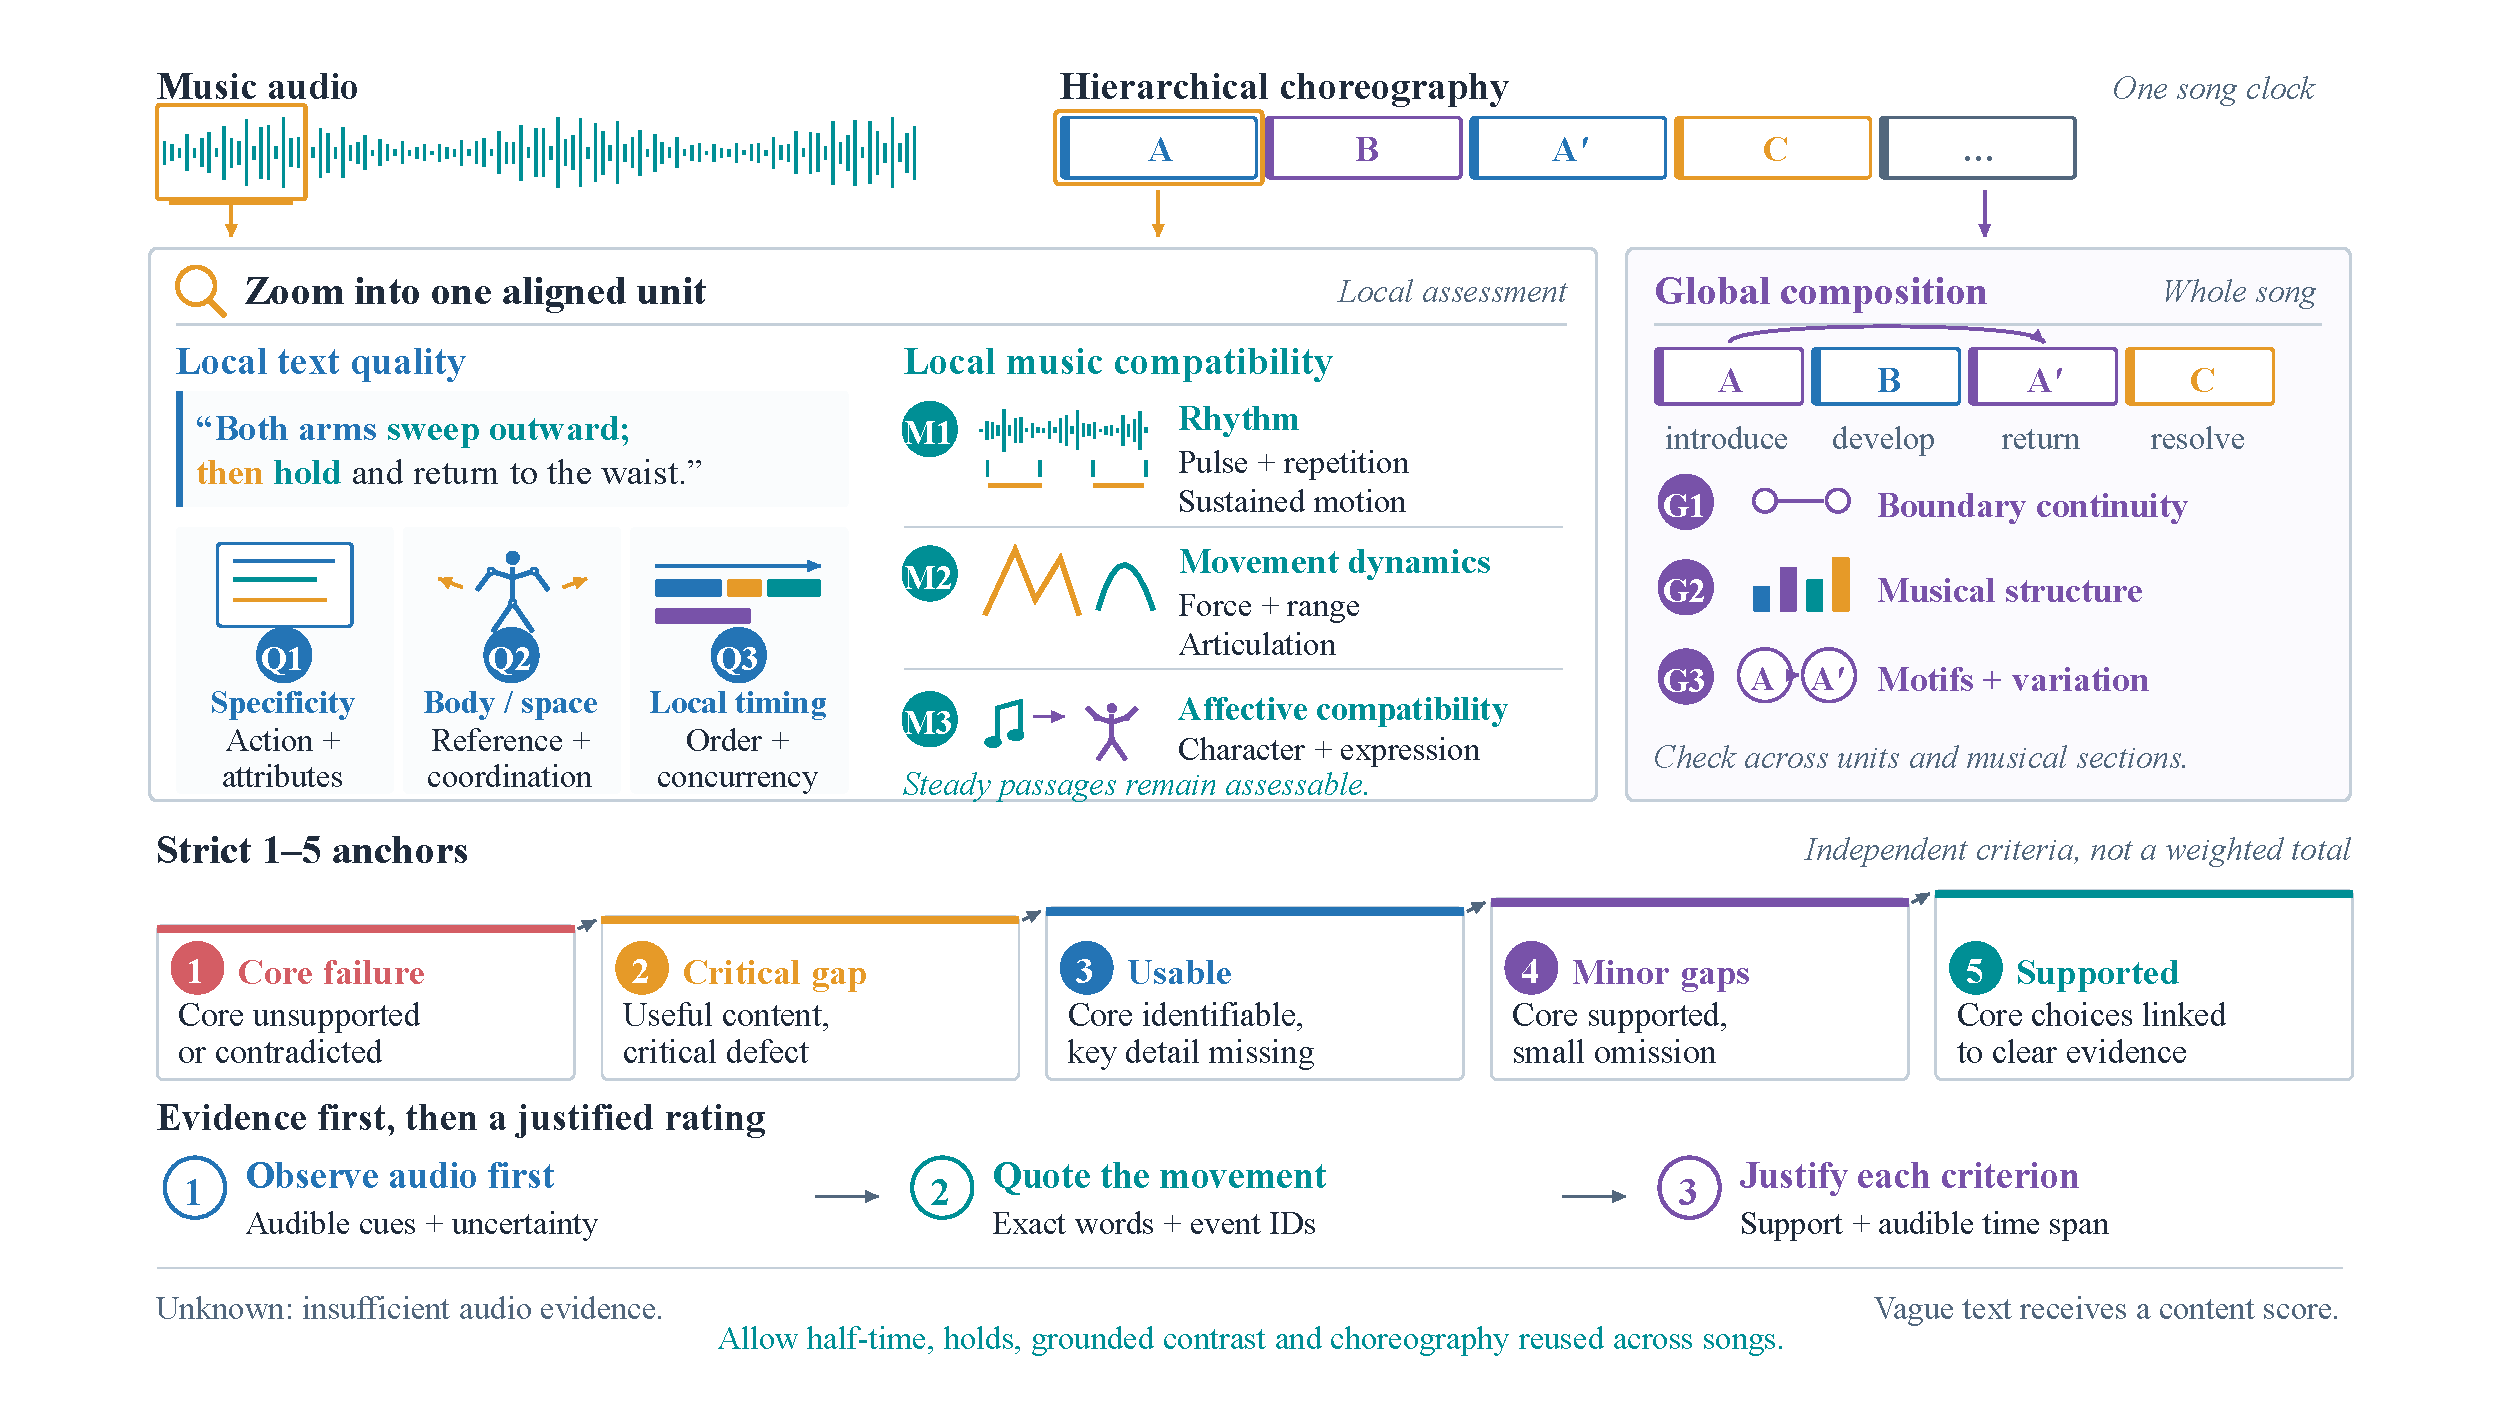
\includegraphics[width=\textwidth]{figures/revision_20261117_v3/paper/evaluation_framework.pdf}
\caption{\textbf{Evidence-grounded evaluation of music and choreography text.}
A single aligned unit supports Q1--Q3 local text quality and M1--M3 music compatibility;
G1--G3 inspect composition across the whole song. The 1--5 anchors require quoted movement
evidence; music-linked claims also require audible support.
M3 assesses affective compatibility, including steady passages.
Unknown denotes insufficient audio evidence, not vague movement text.
Table~\ref{tab:rubric-detailed-anchors} gives the complete guide;
calibration remains pending.}
\label{fig:evaluation-rubric}
\end{figure*}

% Declare the wide results float early so it stays with the main-paper
% experiment discussion rather than being deferred past the conclusion.
% !TeX root = ../main.tex
% Frozen full-2000 aggregates, with BERTScore on the common valid set.
% Requires \usepackage{booktabs}. No model inference was performed.
\begin{table*}[t]
\centering
\caption{Reference agreement on the frozen 2,000-clip choreography panel. BLEU-4 uses a 0--100 scale; other scores are multiplied by 100. BERTScore$^{\dagger}$ uses the common 1,861 valid clips. Higher agreement does not independently establish music alignment or motion quality.}
\label{tab:e2-full2000-v2}
\begingroup
\small
\setlength{\tabcolsep}{3pt}
\renewcommand{\arraystretch}{1.15}
\begin{tabular*}{\textwidth}{@{\extracolsep{\fill}}lrrrrrr@{}}
\toprule
& \multicolumn{4}{c}{Reference text agreement} & \multicolumn{2}{c}{Lexicon agreement}\\
\cmidrule(lr){2-5}\cmidrule(lr){6-7}
Method & BLEU-4 & ROUGE-L & BERT-F1$^{\dagger}$ & Token-F1 & KW-F1 & BP-F1 \\
\midrule
Qwen3-Omni-Instruct & 0.36 & 11.19 & 78.50 & 15.13 & 28.97 & 60.18 \\
MOSS-Audio & 0.73 & 12.77 & 82.64 & 16.32 & 8.76 & 21.31 \\
MOSS-Music & 0.56 & 14.99 & 82.14 & 20.18 & 11.99 & 51.69 \\
Music-Flamingo & 0.85 & 12.79 & 82.29 & 16.11 & 19.67 & 19.46 \\
Audio-Flamingo3 & 0.18 & 7.93 & 82.21 & 9.08 & 9.25 & 12.08 \\
Qwen2.5-Omni & 0.17 & 8.09 & 82.85 & 9.80 & 4.18 & 32.09 \\
\midrule
\textbf{Task-specific SFT (ours)} & \textbf{9.74} & \textbf{30.80} & \textbf{89.71} & \textbf{58.06} & \textbf{80.78} & \textbf{94.12} \\
\bottomrule
\end{tabular*}
\par\vspace{4pt}
\begin{minipage}{\textwidth}\footnotesize
KW/BP: micro-averaged category-set F1 over 39 motion and six body-part
categories. Token-F1: token-multiset overlap. $^{\dagger}$RoBERTa-large,
layer 17, without IDF or baseline rescaling. All remaining metrics use
2,000 clips. Diagnostics and available-case BERTScore appear in
Table~\ref{tab:e2-full2000-diagnostics}. Bold identifies our model.
\end{minipage}
\endgroup
\end{table*}

% Generated by results/build_d123_refinement_table.py from public per-case scores.
\begin{table*}[t]
\centering
\caption{Automatic ratings of our captioning pipeline on a 1--5 scale. r4 and v2.1 are scoring versions applied to the same outputs; v2.1 was defined after earlier tests. Source rating IDs are retained. D4--D6 remain unreported (``--''). Coverage, inference settings, and protocol scope appear in Appendix~\ref{sec:experimental-details}.}
\label{tab:refinement-d123}
\begingroup\small
\setlength{\tabcolsep}{5pt}
\renewcommand{\arraystretch}{1.10}
\begin{tabular*}{\textwidth}{@{\extracolsep{\fill}}llrrrrrr@{}}
\toprule
Method & Rating version & D1 & D2 & D3 & D4 & D5 & D6 \\
\midrule
Ours & r4 & 4.97 & 3.33 & 4.80 & -- & -- & -- \\
Ours & v2.1 & 4.92 & 4.50 & 4.91 & -- & -- & -- \\
\bottomrule
\end{tabular*}
\endgroup
\end{table*}

% Generated by results/build_style_prior_822.py; only the 822-clip population.
\begin{table*}[t]
\centering
\caption{Audio-based dance-style agreement on 822 clips with video-VLM pseudo-labels. MF1: Macro-F1; BA: balanced accuracy. Values are $\times100$; bold marks the highest score per column.}
\label{tab:style-prior-822}
\begingroup\small
\setlength{\tabcolsep}{5pt}
\renewcommand{\arraystretch}{1.08}
\begin{tabular*}{0.90\textwidth}{@{\extracolsep{\fill}}lrrrr@{}}
\toprule
Method & Top-1 & Top-3 & MF1 & BA \\
\midrule
\multicolumn{5}{l}{\emph{Zero-shot audio-language models}} \\
Qwen3-Omni-Instruct & 21.65 & 40.39 & 10.66 & 13.69 \\
MOSS-Audio & 21.17 & 42.70 & 10.41 & 13.79 \\
MOSS-Music & 14.23 & 30.66 & 9.05 & 9.81 \\
Music-Flamingo & 14.23 & 36.01 & 5.07 & 9.00 \\
Audio-Flamingo3 & 12.90 & 38.08 & 2.45 & 8.15 \\
Audio-Flamingo-Next & 15.94 & 25.67 & 5.53 & 10.08 \\
Qwen2.5-Omni & 22.38 & 54.50 & 11.21 & 14.15 \\
\midrule
\multicolumn{5}{l}{\emph{Supervised style heads; frozen MuQ encoder}} \\
MuQ-JEV head: CE & 44.28 & \textbf{81.87} & 29.18 & 29.21 \\
MuQ-JEV head: weighted CE & 41.24 & 77.98 & 29.31 & 30.12 \\
MuQ-JEV head: focal & \textbf{44.77} & 81.39 & \textbf{32.17} & \textbf{32.35} \\
\bottomrule
\end{tabular*}
\endgroup
\end{table*}


\paragraph{Evaluation targets.}
Our music-and-text protocol separates reference agreement, surface
diagnostics, and choreography quality. Connective counts and exact-string
duplication describe surface behavior; neither they nor reference
agreement establish performed synchronization or biomechanics.

\paragraph{Local and whole-song criteria.}
Figure~\ref{fig:evaluation-rubric} groups Q1--Q3 as \emph{local text
quality}, M1--M3 as \emph{local music compatibility}, and G1--G3 as
\emph{global composition}. The figure and
Table~\ref{tab:rubric-detailed-anchors} define integer 1--5 anchors, without
a weighted total: 2 indicates useful content with a critical defect,
3 an important omission, and 4 minor deficiencies. Sustained motion,
half-time, contrast, and intentional recurrence can score highly.
A movement pattern may fit multiple recordings; unique song recovery
is not a quality requirement.
Verbosity and motif labels cannot replace evidence; missing support-foot
information alone is not a contradiction.

\paragraph{Evidence and scoring.}
Ratings require reasons, exact action quotations, and existing event IDs.
M1--M3 and G2--G3 additionally require audible observations with global
timestamps. M3 assesses compatibility between musical character and
bodily expression; it does not require a salient change within a short
window. Ambiguous musical evidence receives \emph{unknown}; a vague
action description instead receives a low score when assessable.
Music observations are obtained before candidates and held fixed across
methods. Service/parsing failures remain separate.

The proposed review contract requires raw responses and checks of types, quotations,
IDs, audio identity, and time bounds. These checks establish format compliance,
not semantic validity, audio coverage, calibration, or listener agreement.

\paragraph{Coverage and aggregation.}
G1--G3 require full-song audio and the complete plan; Q1--Q3 and M1--M3 use crops
with global offsets. A chunk-observation fallback remains unimplemented.

For each method and dimension $d$, $\mathcal V_{sd}$ indexes valid,
assessable regions of song $s$, and $\mathcal S_d$ contains songs with
at least one such region:
\begin{equation}
\label{eq:rubric-aggregation}
\begin{aligned}
\bar r_{sd}&=\frac{1}{|\mathcal V_{sd}|}
                  \sum_{w\in\mathcal V_{sd}}r_{swd},\\
R_d&=\frac{1}{|\mathcal S_d|}\sum_{s\in\mathcal S_d}\bar r_{sd}.
\end{aligned}
\end{equation}
Whole-song dimensions contribute one rating per song. Coverage divides
valid ratings by registered cases, reporting unknown and failed cases
separately. Paired effects use shared valid
regions/songs and song-bootstrap intervals. Completion includes all
registered songs; empty denominators remain undefined.

\paragraph{Controlled validation.}
The prospective controlled protocol fixes beginning/middle/end regions,
evidence, and budgets across Workflow, Self-Refine, ReAct, and our harness.
Calibration and validation require two independent listeners and
cross-family judges. Archived four-criterion, acoustic-summary-only
results (Section~\ref{sec:exp-harness}) assess a different protocol and
cannot validate these audio-conditioned ratings.

% !TeX root = ../main.tex
\section{Experiments}
\label{sec:experiments}

\subsection{Protocol and Evidence Scope}
\label{sec:exp-protocol}
Captioning compares SFT checkpoint 1,000 with six audio-language
baselines~\cite{qwen3omni,mossaudio,mossmusic,musicflamingo,audioflamingo3,qwen25omni}.
All return 2,000 texts; training/checkpoint provenance needs a final
audit before claiming unseen-data generalization. BLEU-4 uses 0--100;
other agreement scores are multiplied by 100. BERTScore uses
RoBERTa-large, layer 17, without IDF or baseline rescaling, on the same
1,861 valid cases for every method; other caption metrics use all 2,000.
Style evaluation uses the 822-clip population only. Automatic caption
ratings use separate versioned protocols. Historical fixed-window
controllers differ from the shared-evidence bar protocol.

\subsection{Short-Clip Caption Agreement}
\label{sec:exp-reference}
SFT leads all six agreement measures (Table~\ref{tab:e2-full2000-v2}),
reaching 9.74 BLEU-4, 30.80 ROUGE-L, and 89.71 BERTScore F1 versus
the strongest baseline values of 0.85, 14.99, and 82.85. This consistency
supports task adaptation; shared references prevent interpreting these
metrics as independent music-quality evidence.

Motion-keyword precision/recall reach 76.23/85.90 versus Qwen3-Omni's
35.09/24.67, showing both broader reference-category coverage and a
lower proportion of non-reference categories. The lexicons omit
laterality, negation, action--body binding, and temporal correctness.
Temporal-connective presence scarcely separates Qwen2.5-Omni
(1,998/2,000) from SFT (2,000/2,000), motivating stricter evidence
requirements. Table~\ref{tab:e2-full2000-diagnostics} retains surface
diagnostics without treating duplication or length as dance quality.

\subsection{Automatic Caption Assessment}
\label{sec:exp-refinement}
Table~\ref{tab:refinement-d123} reports D1--D3 ratings of our captioning
pipeline. Ours obtains 4.97, 3.33, and 4.80 under r4, and 4.92, 4.50,
and 4.91 under v2.1. Means use valid ratings separately for each
dimension; D4--D6 remain unreported.

Both protocols score the same captions, so differences between rows
reflect scoring sensitivity. D1 is near its ceiling: 98.2\% of valid
r4 judgments assign 5. These results describe our system's ratings;
baseline comparisons and independent musical validation remain pending.
Appendix~\ref{sec:experimental-details} documents coverage, the inference
configuration, and the unverified mapping of source rating IDs to our
proposed anchors.

\subsection{Audio-Conditioned Style Prior}
\label{sec:exp-jev}
Table~\ref{tab:style-prior-822} compares three supervised MuQ-JEV
heads with seven zero-shot audio-language models on the same 822 clips.
Rankings use 22 labels, with 13 observed classes and positive training
examples in 15 classes. Focal reaches 44.77 Top-1, 81.39 Top-3,
32.17 Macro-F1, and 32.35 balanced accuracy, versus 22.38, 54.50,
11.21, and 14.15 for the strongest zero-shot comparator, Qwen2.5-Omni.
All three training objectives exceed that comparator on every measure.

Cross-entropy has the highest Top-3 (81.87); focal has the highest
point estimates on the other three metrics. Focal's paired Top-$k$
intervals against cross-entropy include zero. Weighted cross-entropy
trades Top-$k$ accuracy for slightly higher class-balanced scores than
ordinary cross-entropy. These results support supervised style
specialization against video-VLM pseudo-labels. Scarce classes and
incomplete training support limit coverage; human music--dance
suitability and downstream harness benefits require separate evidence.

\subsection{Controller Reliability and Composition}
\label{sec:exp-harness}
% !TeX root = ../main.tex
% Sources: formal_result_v1.json, judge_size_robustness.json,
% extension_set.json in experiments/structured_dev_20261114.
% The extension's attempted=9 and n_paired=8 supersede its stale n=6 field.
\begin{table}[t]
\centering
\caption{Preliminary fixed-window whole-song comparison. Completion reports W/O over all attempts; $n$ counts completed pairs. Entries show O$-$W mean total-score differences and 95\% song-bootstrap intervals. Judges see acoustic summaries and text, not audio; both belong to the planner's Qwen family.}
\label{tab:harness-preliminary}
\begingroup\footnotesize
\setlength{\tabcolsep}{2pt}
\renewcommand{\arraystretch}{1.12}
\begin{tabular*}{\columnwidth}{@{\extracolsep{\fill}}lccrr@{}}
\toprule
Cohort & Completion & $n$ & Qwen 8B & Qwen 30B \\
\midrule
Original & 6/11; 11/11 & 6 & +2.50 & +2.42 \\
 & & & $[0.08,3.92]$ & $[0.00,4.25]$ \\
Extension & 8/9; 9/9 & 8 & +6.00 & +4.44 \\
 & & & $[5.12,6.88]$ & $[3.38,5.56]$ \\
\bottomrule
\end{tabular*}
\endgroup
\end{table}

Only Workflow and Self-Refine complete all 24 songs in the initial
four-policy study (Table~\ref{tab:harness-controller-history}).
Self-Refine uses nearly three times Workflow's calls; tool-loop
policies cost more and complete fewer songs. Additional iteration alone
does not ensure delivery. The old quality check gives all 87 evaluable
plans its maximum, preventing quality discrimination.

The later W/O study uses Qwen3-VL-30B-A3B-Instruct at temperature zero,
approximately 5.06~s windows, and no JEV prior. O adds acoustic guidance
and bounded rewriting with unequal evidence access, a system-level
contrast. Table~\ref{tab:harness-preliminary} separates 11 development
songs from nine subsequent FMA Electronic songs. Completion counts
all attempts; scores use six/eight completed pairs. O completes all
extension songs, whereas W misses one.

Qwen judges favor O by +6.00/+4.44 out of 20 on the extension after
averaging orders. Both see text and acoustic summaries, not audio,
and share the planner's family. Cross-family text-only MOSS yields
$+0.50\;[-1.00,2.00]$, leaving independent musical confirmation
unresolved. These historical scores cannot validate the new rubric
or bar/style mechanisms.

\subsection{Exploratory Mechanism Analysis}
\label{sec:exp-mechanisms}
The repaired four-song comparison (Table~\ref{tab:harness-exploratory})
favors acoustically guided variants under its text-judge setup;
the quota-only interval crosses zero. Unequal evidence and development
reuse preclude isolated component attribution.

Early repair reduces mean normalized exact-text repetition from 73.14\%
to 36.82\% on five valid pairs of six registered songs, all decreasing.
This optimized diagnostic does not establish movement diversity.
Appendix~\ref{sec:remaining-tests} reports presentation sensitivity and
further controls.

% !TeX root = ../main.tex
\section{Conclusion}
\label{sec:conclusion}
\method links source-grounded supervision, a local movement expert,
stateful composition, and evidence-grounded evaluation. Musical units,
committed history, and bounded revision make whole-song decisions
inspectable. Results establish reference agreement and characterize
historical controller reliability; automatic caption ratings also
expose protocol sensitivity. Shared-evidence comparisons and independent
audio-grounded assessment remain necessary to validate the latest
bar-aligned harness.

% !TeX root = ../main.tex
% The factual AI-assistance disclosure is included in the supplementary
% material; the final submission must follow the venue's required location.

\clearpage
% !TeX root = ../main.tex
{\small
\bibliographystyle{ieeenat_fullname}
\bibliography{main}
}


\clearpage
\appendix
\onecolumn
% !TeX root = ../main.tex
\section{Annotation Components and Provenance}
\label{sec:annotation-details}
% !TeX root = ../main.tex
\begin{figure*}[t]
\centering
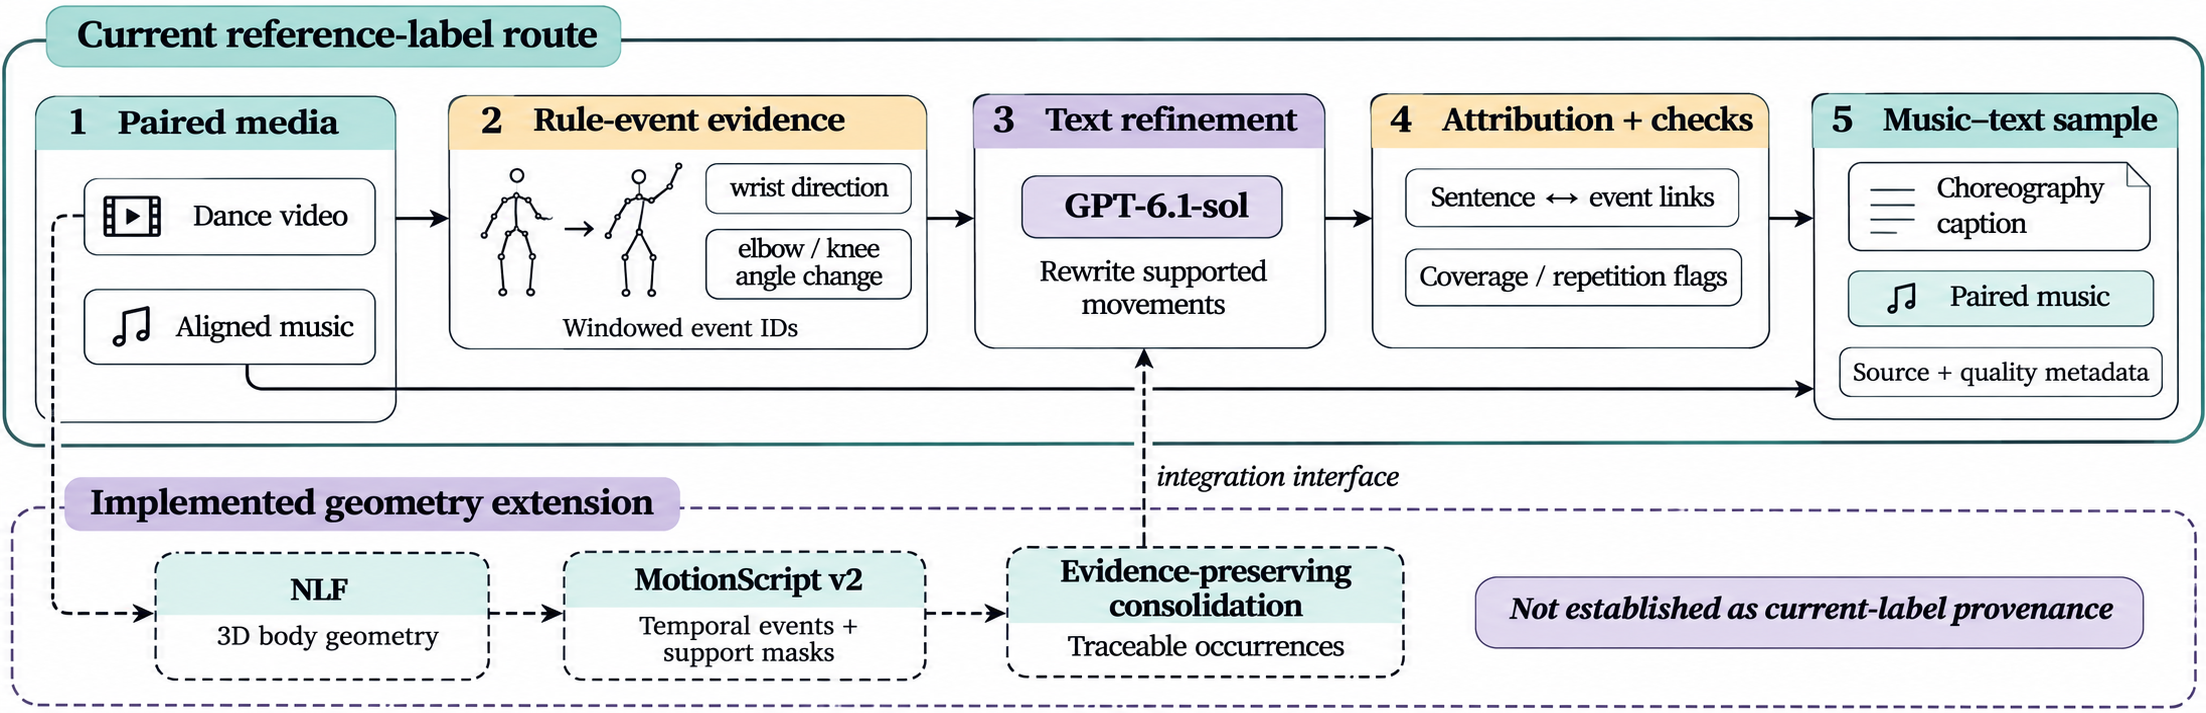
\includegraphics[width=\textwidth]{figures/dataset_construction_gpt_v2.png}
\caption{\textbf{Dataset construction with explicit provenance.}
The solid route produces current reference labels from windowed 2D
rule events through GPT-6.1-sol text refinement, attribution, and
automatic checks. Aligned music bypasses the refiner and is retained
in the final pair. The dashed NLF/MotionScript route is an implemented
extension whose integration into current labels is not established.}
\label{fig:dataset-construction}
\end{figure*}

The main-paper component-integration figure describes the implemented geometric
annotation route and the documented refinement interface. It is not
the established production history of the references used in the
captioning experiment. Those references come from the text-only
refinement of 2D rule-event logs described in Sec.~\ref{sec:data}.
In particular, neither a 20~FPS resampling operation nor additional
template joints introduces a new visual observation.

For descriptive analysis, original annotations and refined captions
were matched by identifier on 22,352 validation/test clips, retaining
all automatic quality flags. Original logs contain 47.21 event
statements per clip on average; refined descriptions contain 135.33
English body words and 5.12 producer-reported sentences. Wrist, elbow,
and knee events account for 60.3\%, 29.7\%, and 10.0\% of source-event
occurrences. These quantities have different units. They do not show
that the number of distinct observed actions increased or that
annotation accuracy improved. Source-style fields are unchanged;
unknown labels remain in the audited population and are reported in
the main text rather than excluded from the statistics.

\section{Composition and Targeted Revision}
\label{sec:revision-details}
% !TeX root = ../main.tex
\begin{figure*}[!htbp]
\centering
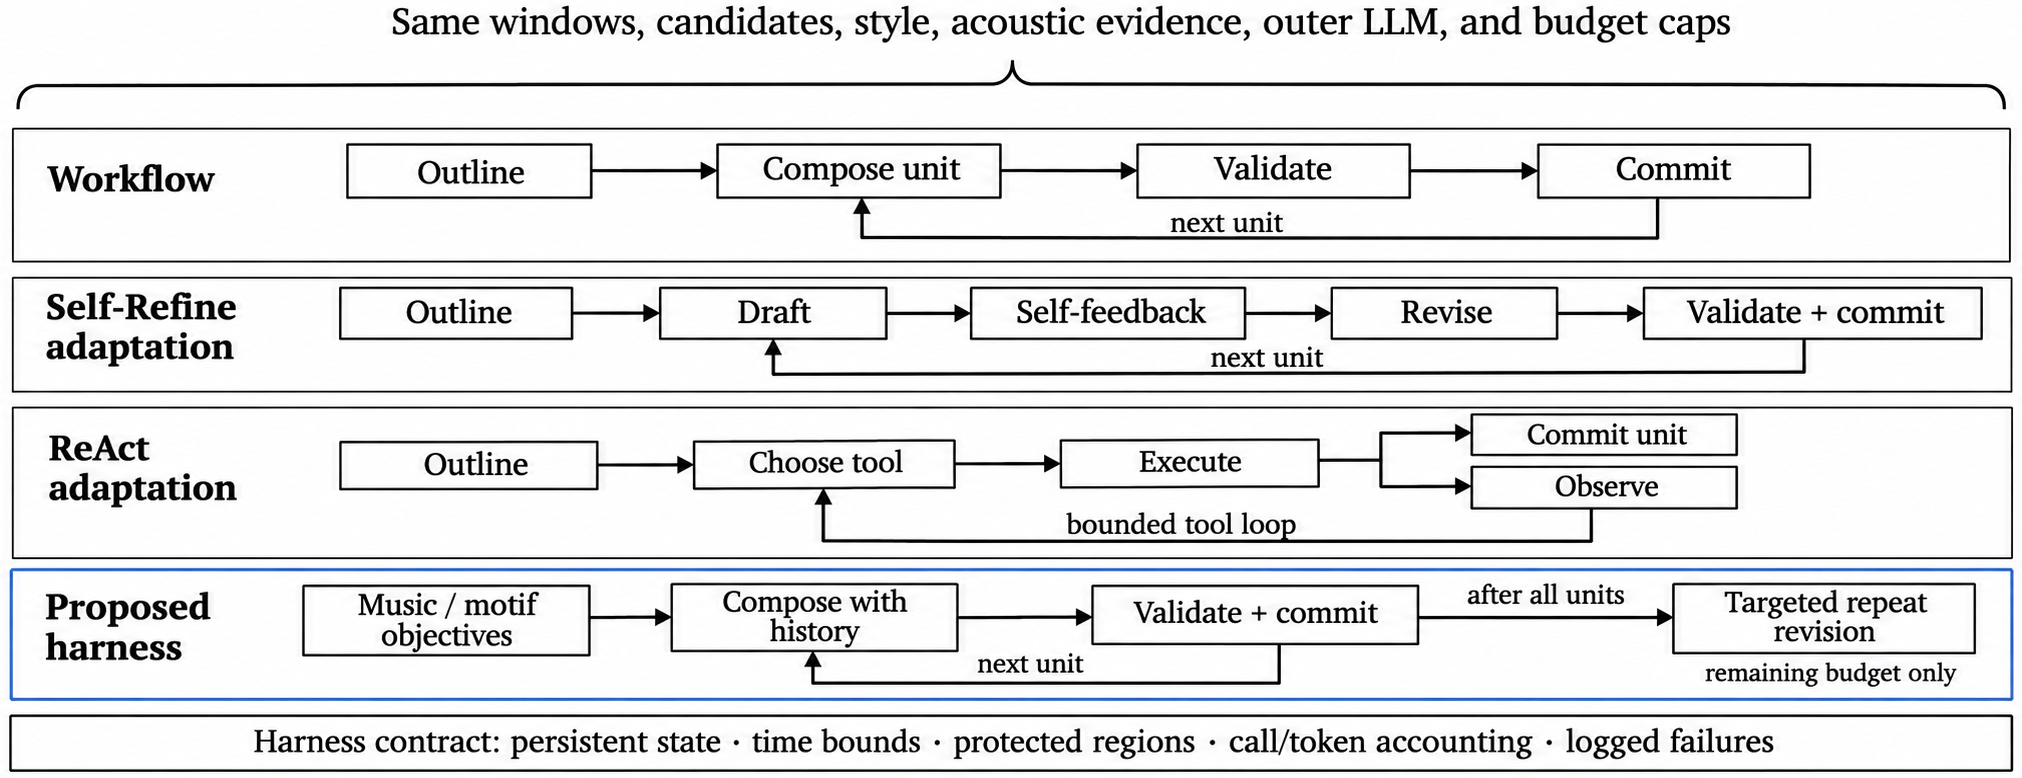
\includegraphics[width=\textwidth]{figures/agent_policy_comparison_gpt.png}
\caption{\textbf{Control-policy schematics for the shared-evidence comparison.}
Workflow uses direct composition, Self-Refine adds per-unit feedback and
revision, and ReAct selects tools through a bounded observation loop.
Commit observations advance ReAct to the next unit within that loop;
the displayed commit branch is a state update, not whole-song termination.
The proposed policy adds music/motif objectives and terminal targeted
revision with remaining budget. Common validation and failure handling
are abbreviated. These are implemented task adaptations, and this
figure reports no comparative quality result.}
\label{fig:agent-policy-comparison}
\end{figure*}

% !TeX root = ../main.tex
% Byte-preserved source and SHA: results/harness/controller_history.provenance.json.
% Historical 20261113 runs; not the current bar-aligned harness.
\begin{table}[t]
\centering
\caption{Earlier fixed-window controllers on 24 songs. Completion counts
legal final plans; mean calls includes all 24 attempts. These runs
predate the current bar-aligned harness.}
\label{tab:harness-controller-history}
\begingroup\footnotesize
\setlength{\tabcolsep}{4pt}
\renewcommand{\arraystretch}{1.08}
\begin{tabular*}{\columnwidth}{@{\extracolsep{\fill}}lrr@{}}
\toprule
Controller & Complete & Calls/song \\
\midrule
Workflow & 24/24 & 24.54 \\
Self-Refine & 24/24 & 71.63 \\
ReAct & 19/24 & 74.88 \\
Early choreography & 20/24 & 76.08 \\
\bottomrule
\end{tabular*}
\endgroup
\end{table}

% !TeX root = ../main.tex
% Provenance: results/harness/exploratory_ablation_repaired.provenance.json
% Use the repaired Section 17 results, not superseded ablation_v1.json.
\begin{table}[t]
\centering
\caption{Exploratory fixed-window ablations after timing repair ($n=4$). Qwen3-VL-8B rates text and acoustic summaries on four criteria (20 points); $\Delta$ is variant$-$W, averaged over orders, with 95\% song-bootstrap intervals. W lacks equal acoustic evidence: these are not isolated component effects or new bar-aligned results.}
\label{tab:harness-exploratory}
\begingroup\small
\setlength{\tabcolsep}{3pt}
\renewcommand{\arraystretch}{1.10}
\begin{tabular*}{\columnwidth}{@{\extracolsep{\fill}}lrr@{}}
\toprule
Variant & $\Delta$ & 95\% CI \\
\midrule
Q: motif quota & $+3.75$ & $[-1.63,\;7.25]$ \\
G: acoustic guidance & $+6.50$ & $[4.75,\;7.75]$ \\
S4: both & $+6.25$ & $[5.50,\;7.00]$ \\
\bottomrule
\end{tabular*}
\endgroup
\end{table}

Figure~\ref{fig:agent-policy-comparison} summarizes the four control
policies. Committed state and the remaining budget persist across unit
boundaries. Reading evidence or checking a draft does not advance the
song; a valid commit does. Only the proposed policy's predeclared
targeted revision stage may patch its selected completed spans.
A repeated movement can be an intentional
motif return. Candidate detection therefore identifies possible
redundancy for constrained revision, rather than determining artistic
quality. The current revision mechanism changes selected action text
while preserving its time bounds and protected regions. Boundary
reasoning remains text-based; it does not reconstruct an unobserved
physical state.

\section{Diagnostic Metrics and Style Protocols}
\label{sec:experimental-details}
% !TeX root = ../main.tex
% Supporting diagnostics; requires booktabs.
\begin{table*}[!htbp]
\centering
\caption{Full-2000 lexicon diagnostics and evaluation coverage. These are supporting statistics, not additional independent choreography-quality experiments.}
\label{tab:e2-full2000-diagnostics}
\begingroup\small
\setlength{\tabcolsep}{3pt}\renewcommand{\arraystretch}{1.12}
\begin{tabular*}{\textwidth}{@{\extracolsep{\fill}}lrrrrrr@{}}
\toprule
\multicolumn{7}{l}{\textbf{A. Micro-averaged lexicon agreement (all values $\times 100$)}}\\
\midrule
Method & KW-P & KW-R & KW-F1 & BP-P & BP-R & BP-F1 \\
\midrule
Qwen3-Omni-Instruct & 35.09 & 24.67 & 28.97 & 50.39 & 74.69 & 60.18 \\
MOSS-Audio & 17.58 & 5.83 & 8.76 & 54.71 & 13.23 & 21.31 \\
MOSS-Music & 15.42 & 9.80 & 11.99 & 49.73 & 53.81 & 51.69 \\
Music-Flamingo & 32.03 & 14.19 & 19.67 & 29.17 & 14.60 & 19.46 \\
Audio-Flamingo3 & 20.00 & 6.02 & 9.25 & 81.67 & 6.52 & 12.08 \\
Qwen2.5-Omni & 7.93 & 2.84 & 4.18 & 72.54 & 20.60 & 32.09 \\
\textbf{SFT v3 (ours)} & \textbf{76.23} & \textbf{85.90} & \textbf{80.78} & \textbf{91.66} & \textbf{96.72} & \textbf{94.12} \\
\bottomrule\end{tabular*}\par\vspace{9pt}
\begin{tabular*}{\textwidth}{@{\extracolsep{\fill}}lrrr@{}}
\toprule
\multicolumn{4}{l}{\textbf{B. BERTScore coverage and original available-case means}}\\
\midrule
Method & Valid / 2,000 & Coverage (\%) & Available-case F1 $\times100$ \\
\midrule
Qwen3-Omni-Instruct & 1,999 & 99.95 & 78.49 \\
MOSS-Audio & 1,999 & 99.95 & 82.63 \\
MOSS-Music & 1,998 & 99.90 & 82.13 \\
Music-Flamingo & 1,865 & 93.25 & 82.29 \\
Audio-Flamingo3 & 2,000 & 100.00 & 82.20 \\
Qwen2.5-Omni & 2,000 & 100.00 & 82.85 \\
SFT v3 (ours) & 2,000 & 100.00 & 89.71 \\
\bottomrule\end{tabular*}\par\vspace{9pt}
\begin{tabular*}{\textwidth}{@{\extracolsep{\fill}}lrrrr@{}}
\toprule
\multicolumn{5}{l}{\textbf{C. Surface diagnostics (no quality ranking)}}\\
\midrule
Method & BV $\times100$ & TC present / 2,000 & Duplicate excess & Length ratio \\
\midrule
Qwen3-Omni-Instruct & 13.03 & 1,721 & 12 & 1.388 \\
MOSS-Audio & 2.01 & 1,996 & 801 & 0.544 \\
MOSS-Music & 10.75 & 1,617 & 16 & 0.995 \\
Music-Flamingo & 7.93 & 1,848 & 626 & 0.750 \\
Audio-Flamingo3 & 0.77 & 1,985 & 1,357 & 0.285 \\
Qwen2.5-Omni & 5.45 & 1,998 & 1,398 & 0.281 \\
SFT v3 (ours) & 43.23 & 2,000 & 0 & 1.063 \\
\bottomrule\end{tabular*}
\par\vspace{5pt}
\begin{minipage}{\textwidth}\footnotesize
\textbf{Reading the diagnostics.} BERT coverage is a measurement-availability statistic, not a quality score. Original means in B use different valid sets and should not be subtracted as paired effects. BV is body-part/verb co-occurrence; TC counts texts containing a temporal connective, not correct temporal relations. Duplicate excess is $N-U$, where $U$ is the number of distinct exact text strings; it is not the count of every sample belonging to a duplicate cluster. A zero does not establish semantic novelty. TC counts and duplicate excess are exact re-expressions of the archived rates, not newly computed semantic metrics. Length ratio is the mean generated/reference character ratio; a value near one is not a quality target. All seven methods returned 2,000 texts. KW and BP inventories are coarse and partly overlapping.
\end{minipage}
\endgroup\end{table*}

The diagnostics retain each method's evaluation coverage and
available-case BERTScore in addition to the common-case main comparison.
An exact duplicate count measures identical returned strings, not
semantic movement diversity. Table~\ref{tab:style-prior-822} reports
only the 822-clip style population, retaining all seven zero-shot models
and all three supervised objectives on the same clips.

\paragraph{Automatic-rating configuration and coverage.}
For Table~\ref{tab:refinement-d123}, \emph{Ours} denotes the supplied
task-specific captioner predictions. Released processing-stage metadata
disagree with the author-reported generation configuration, so the
output-stage lineage remains unresolved. These ratings alone are not
an isolated ablation of supervised fine-tuning.
The Ours release comes from public commit \texttt{dc6dfd9}; the baseline
release comes from \texttt{92d6dcf}. All eight generation inventories
contain the same 2,000 case IDs. All released outputs are retained in
the audit, alongside a separate record of the configuration clarification.
Scores marked invalid or null
are omitted per dimension, never replaced with zero. The public export
contains numeric scores and status fields, without response bodies,
evidence quotations, assessor identity, or acoustic-input metadata.
The main comparison uses the recorded r4 scoring family, the only
published version available for every method. Baselines provide r4
judgments on the same 1,900 holdout IDs; Ours is restricted to those
IDs before aggregation. Each dimension then uses the common valid
intersection across all eight methods: 1,888 for Q1, 1,833 for Q2,
and 1,858 for Q3. The shared valid-case means, per-method available-case
means, missing statuses, and ID hashes are preserved in the audit.
The older baseline v1.2 run is not mixed into the comparison.

For sensitivity on the complete Ours release, r4 yields 4.97/3.33/4.80
and v2.1 yields 4.92/4.50/4.91. v2.1 was defined after earlier tests;
it is excluded from the main comparison because compatible baseline
judgments were not released. No per-dimension maximum across versions
is selected. The baseline manifest identifies the r4 version by name,
but omits the rubric content hash, so exact prompt-hash parity cannot
be independently established from the export.
Published record IDs D1--D3 are displayed as Q1--Q3 without changing
their numerical values. The revised M3 affect criterion replaces the
earlier local-development design; no legacy development scores are reused.
These records cannot establish calibration to our nine-dimensional
anchors. Differences between protocols are not model improvements, and
reference agreement has not been recomputed on the supplied rating outputs.
Full-release Ours Q1/Q2/Q3 valid counts are 1,999/1,990/1,999 for r4
and 2,000/1,966/1,999 for v2.1; these available-case values are not
substituted for the common-case main table. The earlier two-axis
baseline assessment is likewise not relabeled as these three dimensions.

\paragraph{Caption decoding and metric configuration.}
Reference agreement uses 2,000 clips; BERTScore uses the common
1,861 valid cases for every method, while the other main-table reference
metrics use all clips.
The reported SFT checkpoint uses temperature 0.7, top-$p$ 0.9,
top-$k$ 20, one beam, repetition penalty 1.05, no-repeat 4-grams,
at most 1,024 generated tokens, and an explicit chat EOS. A per-case
sampling seed is derived from its identifier. The baseline stopping
metadata are incomplete; a returned text does not by itself prove
that generation was untruncated. BERTScore is computed without silent
truncation on the common valid intersection; the available-case
statistics use different case sets and cannot be subtracted as paired
effects.

\paragraph{Style pseudo-labels and supervision.}
The 822-clip style population uses video-VLM pseudo-labels, rather than
human judgments of music--dance suitability. Rankings use 22 labels;
Macro-F1 and balanced accuracy average over the 13 classes observed in
this population. Eight classes have 100 examples each; the other five
have 1, 1, 1, 3, and 16 examples. Class-balanced scores are therefore
descriptive and sensitive to very scarce classes.

The frozen MuQ encoder supplies features to three supervised heads:
cross-entropy, weighted cross-entropy, and focal loss. Positive training
examples cover only 15 of 22 outputs. Focal was selected by validation
Macro-F1, then balanced accuracy and unweighted NLL, before inspecting
this preview; scalar-temperature calibration uses separate calibration
data. The paired focal-minus-cross-entropy 95\% intervals are
$[-2.43,3.53]$ points for Top-1 and $[-2.68,1.70]$ for Top-3.
Seven unsupported outputs prevent a complete 22-class training claim.
Neither classification agreement nor these objective comparisons establish
that conditioning a harness on the predicted style improves choreography.

\section{Implementation and Validation Details}
\label{sec:remaining-tests}
% !TeX root = ../main.tex
\paragraph{Observation and planning contracts.}
The candidate cache retains the source audio identity, exact observation
intervals, model configuration, and generation provenance. Proposals
are compositional evidence rather than ground-truth action sequences
or instructions that must be copied verbatim. Extending the planning
horizon does not require the captioner to describe an entire song in
one response. The outline and committed history supply long-range
context beyond local proposals.

\paragraph{Reproducible controller defaults.}
The candidate collector defaults to two proposals per observation window.
The controlled experiment runner uses up to five repetition groups;
older runs may use the underlying controller's three-group default and
must retain their recorded configuration. Grouping compares normalized
token sets against a representative action at Jaccard similarity
$\geq0.80$. The first occurrence stays fixed. Replacement text is accepted
only when its overlap with the representative lies between 0.20 and
0.80 and the patch passes structural validation. This vocabulary guard
does not verify semantic correctness. Each selected group receives at
most one request within the remaining outer budget. Time, track, motif,
evidence, and other protected event fields remain unchanged.

\paragraph{Clock and cost accounting.}
Observation and event boundaries use integer samples on the canonical
audio clock. Exported review cases divide these boundaries by the source
sample rate to obtain global seconds, retaining the original offset for
audio crops. Shared audio preparation and candidate collection are
accounted for separately from outer composition. The $1+4U$ outer-call
limit is an upper bound, not a fixed inference cost. Client-visible
dispatches and their usage are recorded; any hidden service retry
requires separate tracing before physical-request totals can be claimed.
The cached proposal and evidence configuration is fixed for the new
controlled comparison, while historical results retain their original
conditions.

\paragraph{Variable-duration deployment.}
The bar partition supplies both observation intervals and planning units.
Leading and trailing incomplete bars remain explicit fragments; a short
fragment may merge with a neighbor in the same public section.
Insufficient downbeat evidence or an unsupported duration requires
review rather than silent fallback to fixed windows. Audio is neither
stretched nor implicitly truncated to match the target duration.
Variable-duration captioner consumption requires server preflight:
successful partitioning and waveform loading do not establish that the
model's processor consumes the entire waveform or preserves caption
quality. The current variable-duration collection path uses a native
model resident in one process; the legacy fixed-duration service
contract cannot substitute for this path. These deployment checks have
not yet been reported as completed model experiments.

\paragraph{Global condition and evidence.}
The style predictor may retain its native short observation windows
independently of the choreography partition. Duration-weighted pooling
gives overlapping observations shared ownership of their common span.
The resulting label is a creative prior rather than a unique correct
dance genre. The composer consumes cached captions and acoustic
summaries; it has no additional raw-audio listening tool inside the
current composition loop. An unavailable or uncertain signal must remain
explicit rather than be replaced with an invented musical label.

\paragraph{Scoped editing interface.}
For editing, the user supplies an instruction and target regions or
event identifiers. A version-bound patch declares editable targets,
protected fields, and any explicitly permitted boundary-repair events.
Changes outside this scope are rejected; accepted operations are
applied transactionally and the resulting score is validated. This
protects unrelated choreography, while semantic fulfillment of the
request requires separate evaluation. The interface does not establish
the physical feasibility of an unrendered dance, and a validated
user-editing experiment is not included in the current results.

The controlled comparison preserves failed and partial runs in its
registered inventory. It requires no additional model training.

Two implemented revision controls reuse the actual saved drafts:
the proposed harness before its terminal revision, and the Workflow
draft passed through the same revision mechanism with its remaining
budget. They isolate structured composition from simply adding more
rewriting. Further ablations can compare true bar-aligned versus fixed
windows, remove the global style condition, or permute acoustic evidence
from an immutable source copy. They require independent runs and are
not assigned numerical outcomes in this draft.

The latest implementation has static syntax and consistency checks;
its real variable-duration model input and audio-judge coverage still
require server validation. The 2,000-clip reference panel also needs a
final training/checkpoint provenance audit before it can support a
strictly unseen-data generalization claim. The evaluation report names
the v3 base model and joint-aware clause weighting. The released
implementation and checkpoint report specify a lower-limb vocabulary
and a coefficient of 1.5. The original run configuration and source
hashes are still needed to verify the exact training scope, optimizer
schedule, batch size, and record filter. A controlled comparison
against trained-model-disabled decoding would further isolate the
effect of adaptation. A listener study, rubric sensitivity controls,
and human--model agreement are needed before the new rubric can be
presented as a validated automatic quality metric.

\paragraph{Joint-aware clause reweighting.}
The released configuration targets clauses naming leg, knee, thigh,
shin, calf, hamstring, or quad. Clause boundaries follow commas,
semicolons, and sentence stops. With tokenizer offsets, all overlapping
clause tokens receive the weight; an offset-mapping fallback marks
matched part tokens only. Weighted cross-entropy is normalized by the
unweighted number of valid assistant tokens, not by the sum of weights.
The development report records lower-limb mention coverage of 0.993
in references versus 0.787 in baseline outputs, motivating the selected
region. These are lexical diagnostics, not joint-motion accuracy.
A random-clause control has not been run, so version differences cannot
be attributed solely to the semantics of the selected joints.

\paragraph{Reference-metric calculation.}
For a predicted category set $P_i$ and reference set $R_i$, the pooled
counts are $\mathrm{TP}=\sum_i|P_i\cap R_i|$,
$\mathrm{FP}=\sum_i|P_i\setminus R_i|$, and
$\mathrm{FN}=\sum_i|R_i\setminus P_i|$. The reported lexicon score is
\begin{equation}
 F_{1,\mathrm{micro}}=
 \frac{2\mathrm{TP}}{2\mathrm{TP}+\mathrm{FP}+\mathrm{FN}}.
\end{equation}
The same definition is applied separately to the motion-keyword and
body-part inventories; it is not a score for binding the two. Token-F1
uses token multiplicity rather than binary category membership.
ROUGE-L uses longest-common-subsequence overlap; BERTScore uses
contextual token matching. Corpus BLEU-4 is displayed after multiplication
by 100, so a table value above one is consistent with its scale.
There is no additional undocumented normalized-BERT composite in the
main comparison. BERTScore's raw F1 and its valid-case coverage are
reported explicitly.

\paragraph{Plan diagnostics.}
For a song of duration $T$ and written action intervals $I_k$, temporal
coverage is $|\bigcup_k(I_k\cap[0,T])|/T$. This measures how much time
has a scheduled description, not whether the dancer follows the beat.
Exact duplicate excess is $N-U$, where $U$ is the number of unique
returned strings. Near-text similarity identifies potential repeated
wording; neither measure can distinguish a desirable recurring motif
from unproductive copying without context. Confirmed boundary conflicts
should count only explicit incompatible states and report the number
of boundaries for which sufficient evidence exists.

\paragraph{Historical mechanism diagnostics.}
The earlier repetition-repair experiment counts normalized exact
strings within each plan: $d_s=1-U_s/N_s$, where $N_s$ is its number
of action entries and $U_s$ its number of unique normalized strings.
Normalization lowercases text, replaces non-alphanumeric characters
with spaces, and collapses whitespace. The main-text 73.14\% and 36.82\%
are means over five paired song records, not a pooled event-level rate;
the sixth registered record has no valid pair. This early variant
rewrites at most three groups. It differs from both the cosine-based
near-duplicate diagnostic and the latest five-group Jaccard-based
revision mechanism. Their rates cannot be combined.

The repaired four-song ablation supersedes the earlier timing-unit
results. Its songs participated in development, and the archived
summary does not fully establish label blinding and action-text
presentation limits. We retain its uncertainty intervals as exploratory
evidence. In a separate six-song presentation audit, extending visible
action text from 160 to 400 characters removes the apparent advantage
of more restrictive rewriting over its predecessor: $0.00\;[-2.00,2.00]$.
This is a sensitivity result, not confirmation of equivalent quality.
An identical-plan control has seven parsed pairs of eight registered;
its two-order mean difference is zero, but six of 56 dimension-level
comparisons still favor a presentation position. Order averaging
therefore does not establish an unbiased judge.

\paragraph{Quality summaries and uncertainty.}
The proposed rubric keeps each dimension separate. For local evaluation,
the three common regions are first averaged within each song using the
scored regions for that dimension. A song-level mean then gives each
song equal weight, with valid-region and valid-song counts reported.
Unknown judgments are not replaced by zeros.
Comparisons use paired song differences; source-group bootstrap draws
resample songs together with all of their regions. The planned primary
comparisons are the proposed method against each of the three baseline
policies on G1--G3; multiplicity control and the primary judge must be
frozen before examining results. These aggregation rules specify the
next experiment and do not imply that new rubric scores already exist.

\section{Limitations and Responsible Use}
The current labels inherit the observational limits of their source
events and do not supply unique correct dances for music. Projected
directions do not always identify anatomical laterality. Missing or
occluded body regions can produce uncertain geometry, and richer
wording must not be interpreted as new visual evidence. The global
style classifier is a supervised creative prior evaluated against
video-derived pseudo-labels; it is neither a universal music-genre
classifier nor an authority on culturally appropriate choreography.

The outer composer uses summarized evidence, rather than direct raw
audio in its tool loop. Its checks verify a written schedule and
explicit textual constraints, not balance, joint limits, contact, or
injury risk. Precise editing is supported by scoped permissions, but a
validated user-editing experiment is not included here. Dataset release
must respect the licenses and permissions of the underlying music and
videos; these rights cannot be inferred from the availability of
derived captions.

\section{Detailed Rubric and Calibration Guide}
\label{sec:rubric-guide}
% !TeX root = ../main.tex
% Condensed from tables/rubric_anchors_detailed.tex; no additional scoring standard.
\begin{table*}[t]
\centering
\caption{Core anchors of the proposed rubric. Scores 1 and 5 require dimension-specific evidence; intermediate anchors and exceptions appear in Table~\ref{tab:rubric-detailed-anchors}. Calibration remains pending.}
\label{tab:rubric-core-anchors}
\begingroup\small
\setlength{\tabcolsep}{4pt}
\renewcommand{\arraystretch}{1.10}
\begin{tabular}{@{}>{\raggedright\arraybackslash}p{0.15\textwidth}>{\raggedright\arraybackslash}p{0.405\textwidth}>{\raggedright\arraybackslash}p{0.405\textwidth}@{}}
\toprule
Dimension & 1: core failure & 5: supported fulfillment \\
\midrule
D1: Specificity & Mood/style or generic dancing leaves the main movement unidentifiable. & Main movements and necessary attributes are explicit, without inventing the action. \\
D2: Body/space & Explicit body, spatial, reference-frame, or concurrent-action relations conflict. & Necessary body/spatial relations are clear and compatible, including concurrent actions. \\
D3: Local timing & Order/duration conflicts; clearly serial actions exceed available time. & Order, concurrency, sustained actions, and transitions fit the interval coherently. \\
D4: Rhythm & Claimed rhythm contradicts audible pulse/pauses, or movement rhythm is unspecified. & Repetition, pauses, speed, or movement density correspond to audible rhythm. \\
D5: Expression & Claimed force/articulation conflicts with, or depends on absent, audible features. & Force, articulation, or sustained motion responds to audible expression or grounded contrast. \\
D6: Development & Invents a key musical change, or an applicable change lacks a movement response. & Movement maintenance, emphasis, or change relates to independently identified musical development. \\
\midrule
L1: Continuity & Important boundaries impose incompatible explicit states without a resolving transition. & Important boundaries connect coherently, without decisive explicit state conflicts. \\
L2: Global structure & Unorganized concatenation or explicit conflict with audible whole-song structure. & Section functions and overall progression coherently reflect musical development. \\
L3: Motifs/variation & Unorganized repetition or unrelated changes prevent recognizable thematic development. & Recognizable motifs recur, extend, or vary at musically justified positions. \\
\bottomrule
\end{tabular}
\endgroup
\end{table*}

% !TeX root = ../main.tex
% Dimension definitions: notes/54_benchmark_rubric_ablations_and_case_studies_20261114_zh.md.
% Executable identifiers/common scale: experiments/structured_dev_20261114/judge_rubric_v2.py.
% This table is a recommended calibration guide, not a completed validation study.
\begin{table}[!htbp]
\centering
\caption{Detailed anchors for the proposed evaluation protocol. The executor implements the nine dimension identifiers and common 1--5 scale. The dimension-specific anchors below are a \textbf{recommended calibration guide}, not validated scoring thresholds or completed calibration results. Judge only the supplied music and timed action text.}
\label{tab:rubric-detailed-anchors}
\begingroup\small
\setlength{\tabcolsep}{4pt}
\renewcommand{\arraystretch}{1.11}
\begin{tabular}{@{}>{\raggedright\arraybackslash}p{0.13\textwidth}p{0.27\textwidth}p{0.27\textwidth}p{0.27\textwidth}@{}}
\toprule
Dimension & 1: severe defect & 3: usable but important omission & 5: supported fulfillment \\
\midrule
D1: Movement specificity & Core movement cannot be identified; text mainly states mood, style, or generic dancing. & Main movement is identifiable, but an attribute essential to interpreting it is missing. & Core movements and necessary attributes are explicit, without requiring the reader to invent the main action. \\
\addlinespace
D2: Body/spatial consistency & Explicit body-part, laterality, reference-frame, or simultaneous-action relations conflict. & Most relations are understandable, but an important direction, referent, or coordination relation is ambiguous. & Necessary body/spatial relations are clear and mutually consistent; simultaneous actions are compatible as written. \\
\addlinespace
D3: Local temporal organization & Explicit order, concurrency, or duration requirements conflict, or clearly serial actions exceed the available time. & The local sequence is intelligible, but a consequential duration, transition, or temporal dependency is underspecified. & Ordering, concurrency, sustained actions, and transitions fit the stated interval without an explicit timing conflict. \\
\addlinespace
D4: Rhythmic response & Asserted rhythmic correspondence contradicts audible pulse/pauses, or no assessable movement rhythm is specified. & Movement rhythm broadly fits, but its connection to a specific audible pattern is weak or incomplete. & A concrete relationship links movement repetition, pauses, speed, or density to audible rhythm; justified half-time remains valid. \\
\addlinespace
D5: Expressive response & Claimed force or articulation correspondence relies on an absent musical feature or a clear unsupported conflict. & The broad expression is compatible, but movement force, release, articulation, or its musical rationale remains generic. & Specific force, articulation, or sustained movement responds to audible expression, including a clearly grounded intentional contrast. \\
\addlinespace
D6: Local development response & Invents a key musical change, or an applicable change has no interpretable movement response. & Some movement development is described, but its relation to the independently identified musical change is incomplete. & Maintaining, emphasizing, or changing movement has a clear relationship to the independently identified audible development. \\
\midrule
L1: Cross-window continuity & Important neighboring windows impose explicitly incompatible states with no resolving transition. & Most boundaries connect, but an important transition remains ambiguous or insufficiently explained. & Important boundaries admit coherent transitions; no decisive explicit state conflict remains across neighboring windows. \\
\addlinespace
L2: Global development & The score is predominantly unorganized concatenation or clearly conflicts with the audible whole-song structure. & A global arrangement exists, but section roles, contrast, or progression are weakly connected. & Section functions and overall progression form a coherent plan grounded in the music's actual development. \\
\addlinespace
L3: Motif recurrence/variation & Templates repeat without musical organization, or unrelated changes prevent recognizable thematic development. & Recognizable motifs and variation occur, but some returns or changes lack a clear organizing rationale. & Recognizable motifs recur, extend, or vary at musically justified positions; repeated material has a coherent purpose. \\
\bottomrule
\end{tabular}
\par\vspace{5pt}
\begin{minipage}{\textwidth}\footnotesize
\textbf{Intermediate scores.} Score 2 retains some useful content but has a critical defect; score 4 meets core requirements with only minor deficiencies. Scores 4--5 require a concrete correspondence, not generic claims of suitability. One defect affects multiple dimensions only when its consequences independently warrant each deduction.
\par\smallskip
\textbf{Evidence.} Every numeric score requires an exact quotation, cited event identifiers, and a reason. D4--D6 and L2--L3 additionally require an audible observation and an interval on the global song clock. Quote matching and timestamp validation check the response contract, not semantic correctness or actual model listening.
\par\smallskip
\textbf{Unknown and applicability.} Insufficient observable evidence gives \emph{unknown}, with no numeric score; assessable vagueness or poor content instead receives a low score. Only D6 permits \emph{not applicable}, when its audio-only applicability decision was frozen as false before candidates were inspected. Unresolved D6 applicability gives unknown for every method. Missing audio, service errors, and parsing failures retain distinct failure records and count toward coverage reporting.
\par\smallskip
\textbf{Creative latitude.} Do not require extra joints, longer descriptions, faster movement, or a change at every musical event. Sustained movement, silence, half-time, contrast, and motivated repetition are legitimate. An unspecified support foot alone is not an explicit contradiction. D3 concerns the written local schedule; L1 concerns boundaries between windows. Neither measures biomechanics of an executed dance.
\end{minipage}
\endgroup
\end{table}

The anchors distinguish requirements for local movement, music response,
and whole-song organization. Before collecting formal scores, calibration
should test claim-specific musical contrasts, compatible cross-song reuse,
explicit body/timing conflicts, unproductive copying, and legitimate motif
returns on frozen examples. A choreography need not identify a unique song.
Neither a visually clear rubric nor successful response validation
establishes agreement with independent listeners.

\paragraph{AI assistance.}
Language models assisted with drafting and revising manuscript text,
literature organization, code, and experiment planning. GPT Image
produced early conceptual illustrations; the current diagrams were rebuilt
as editable vector objects, and statistical panels reproduce frozen
audit values. GPT-6.1-sol participates in annotation refinement.
Numerical results come from saved experiment artifacts. The authors
retain responsibility for the manuscript, citations, figures, code,
data provenance, results, and final submission declarations.


\end{document}
